% Chapter X

\chapter{Valutazione del metodo rispetto alle linee ferroviarie} 
Ciascuna delle tratte è stata suddivisa in sotto-tratte lunghe 1500 metri. Ogni sotto-tratta è stata ulteriormente campionata con un passo di 300 metri. Sia le sotto-tratte che i punti derivanti dal campionamento sono stati fatti afferire alle classi alta, medio e basa introdotte nel capitolo \ref{ch:validazione_stazioni}.
Una visione d'insieme dei risultati sull'exposure delle tratte è data in figura \ref{tratte_exposure}. La colorazione delle tratte rispecchia le classi di exposure. 

\begin{figure}[h]
	\centering
	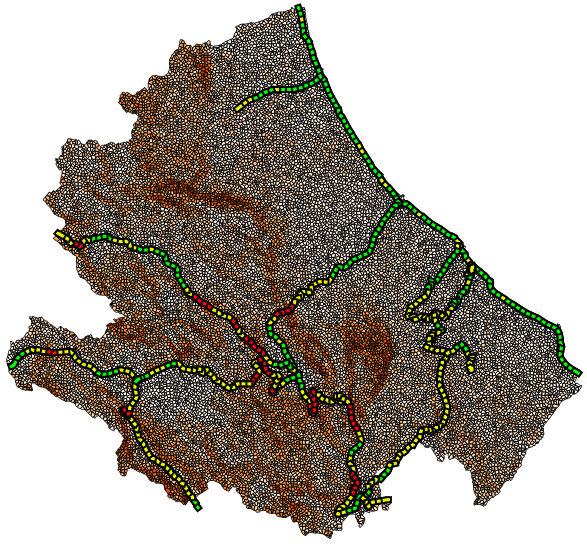
\includegraphics[width=0.8\textwidth]{images/completo}
	\caption{Exposure tratte regione Abruzzo.}
	\label{tratte_exposure}
\end{figure}

Nelle prossime sezioni verranno esposti i risultati di ciascuna tratta con un analisi approfondita della Rieti - L'Aquila - Sulmona.

\section{Bologna - Bari}
La tratta Bologna - Bari non ha sotto-tratte con exposure elevate. Infatti nessuna rientra nella classe alta (Tabella \ref{exposure_sotto_tratte_bologna_bari}).
\tiny
\begin{table}[H]
	\centering
	\begin{tabular}{
			>{\columncolor[HTML]{32CB00}}l 
			>{\columncolor[HTML]{32CB00}}l l
			>{\columncolor[HTML]{32CB00}}l 
			>{\columncolor[HTML]{32CB00}}l l
			>{\columncolor[HTML]{32CB00}}l 
			>{\columncolor[HTML]{32CB00}}l lll}
		\multicolumn{1}{c}{\cellcolor[HTML]{C0C0C0}\textbf{Km}} & \multicolumn{1}{c}{\cellcolor[HTML]{C0C0C0}\textbf{Exposure}} & \multicolumn{1}{c}{\cellcolor[HTML]{C0C0C0}\textbf{}} & \multicolumn{1}{c}{\cellcolor[HTML]{C0C0C0}\textbf{Km}} & \multicolumn{1}{c}{\cellcolor[HTML]{C0C0C0}\textbf{Exposure}} & \multicolumn{1}{c}{\cellcolor[HTML]{C0C0C0}\textbf{}} & \multicolumn{1}{c}{\cellcolor[HTML]{C0C0C0}\textbf{Km}} & \multicolumn{1}{c}{\cellcolor[HTML]{C0C0C0}\textbf{Exposure}} & \multicolumn{1}{c}{\cellcolor[HTML]{C0C0C0}\textbf{}} & \multicolumn{1}{c}{\cellcolor[HTML]{C0C0C0}\textbf{Km}} & \multicolumn{1}{c}{\cellcolor[HTML]{C0C0C0}\textbf{Exposure}} \\ \cline{1-2} \cline{4-5} \cline{7-8} \cline{10-11} 
		\multicolumn{1}{|l|}{\cellcolor[HTML]{32CB00}123}       & \multicolumn{1}{l|}{\cellcolor[HTML]{32CB00}0,00}             & \multicolumn{1}{l|}{}                                 & \multicolumn{1}{l|}{\cellcolor[HTML]{32CB00}19,5}       & \multicolumn{1}{l|}{\cellcolor[HTML]{32CB00}0,02}             & \multicolumn{1}{l|}{}                                 & \multicolumn{1}{l|}{\cellcolor[HTML]{32CB00}7,5}        & \multicolumn{1}{l|}{\cellcolor[HTML]{32CB00}0,10}             & \multicolumn{1}{l|}{}                                 & \multicolumn{1}{l|}{\cellcolor[HTML]{32CB00}22,5}       & \multicolumn{1}{l|}{\cellcolor[HTML]{32CB00}0,15}             \\ \cline{1-2} \cline{4-5} \cline{7-8} \cline{10-11} 
		\multicolumn{1}{|l|}{\cellcolor[HTML]{32CB00}18}        & \multicolumn{1}{l|}{\cellcolor[HTML]{32CB00}0,00}             & \multicolumn{1}{l|}{}                                 & \multicolumn{1}{l|}{\cellcolor[HTML]{32CB00}91,5}       & \multicolumn{1}{l|}{\cellcolor[HTML]{32CB00}0,03}             & \multicolumn{1}{l|}{}                                 & \multicolumn{1}{l|}{\cellcolor[HTML]{32CB00}36}         & \multicolumn{1}{l|}{\cellcolor[HTML]{32CB00}0,10}             & \multicolumn{1}{l|}{}                                 & \multicolumn{1}{l|}{\cellcolor[HTML]{32CB00}85,5}       & \multicolumn{1}{l|}{\cellcolor[HTML]{32CB00}0,16}             \\ \cline{1-2} \cline{4-5} \cline{7-8} \cline{10-11} 
		\multicolumn{1}{|l|}{\cellcolor[HTML]{32CB00}45}        & \multicolumn{1}{l|}{\cellcolor[HTML]{32CB00}0,00}             & \multicolumn{1}{l|}{}                                 & \multicolumn{1}{l|}{\cellcolor[HTML]{32CB00}6}          & \multicolumn{1}{l|}{\cellcolor[HTML]{32CB00}0,03}             & \multicolumn{1}{l|}{}                                 & \multicolumn{1}{l|}{\cellcolor[HTML]{32CB00}67,5}       & \multicolumn{1}{l|}{\cellcolor[HTML]{32CB00}0,10}             & \multicolumn{1}{l|}{}                                 & \multicolumn{1}{l|}{\cellcolor[HTML]{32CB00}15}         & \multicolumn{1}{l|}{\cellcolor[HTML]{32CB00}0,16}             \\ \cline{1-2} \cline{4-5} \cline{7-8} \cline{10-11} 
		\multicolumn{1}{|l|}{\cellcolor[HTML]{32CB00}66}        & \multicolumn{1}{l|}{\cellcolor[HTML]{32CB00}0,00}             & \multicolumn{1}{l|}{}                                 & \multicolumn{1}{l|}{\cellcolor[HTML]{32CB00}99}         & \multicolumn{1}{l|}{\cellcolor[HTML]{32CB00}0,03}             & \multicolumn{1}{l|}{}                                 & \multicolumn{1}{l|}{\cellcolor[HTML]{32CB00}57}         & \multicolumn{1}{l|}{\cellcolor[HTML]{32CB00}0,10}             & \multicolumn{1}{l|}{}                                 & \multicolumn{1}{l|}{\cellcolor[HTML]{32CB00}0}          & \multicolumn{1}{l|}{\cellcolor[HTML]{32CB00}0,16}             \\ \cline{1-2} \cline{4-5} \cline{7-8} \cline{10-11} 
		\multicolumn{1}{|l|}{\cellcolor[HTML]{32CB00}46,5}      & \multicolumn{1}{l|}{\cellcolor[HTML]{32CB00}0,00}             & \multicolumn{1}{l|}{}                                 & \multicolumn{1}{l|}{\cellcolor[HTML]{32CB00}102}        & \multicolumn{1}{l|}{\cellcolor[HTML]{32CB00}0,04}             & \multicolumn{1}{l|}{}                                 & \multicolumn{1}{l|}{\cellcolor[HTML]{32CB00}87}         & \multicolumn{1}{l|}{\cellcolor[HTML]{32CB00}0,11}             & \multicolumn{1}{l|}{}                                 & \multicolumn{1}{l|}{\cellcolor[HTML]{32CB00}96}         & \multicolumn{1}{l|}{\cellcolor[HTML]{32CB00}0,16}             \\ \cline{1-2} \cline{4-5} \cline{7-8} \cline{10-11} 
		\multicolumn{1}{|l|}{\cellcolor[HTML]{32CB00}28,5}      & \multicolumn{1}{l|}{\cellcolor[HTML]{32CB00}0,00}             & \multicolumn{1}{l|}{}                                 & \multicolumn{1}{l|}{\cellcolor[HTML]{32CB00}93}         & \multicolumn{1}{l|}{\cellcolor[HTML]{32CB00}0,04}             & \multicolumn{1}{l|}{}                                 & \multicolumn{1}{l|}{\cellcolor[HTML]{32CB00}78}         & \multicolumn{1}{l|}{\cellcolor[HTML]{32CB00}0,11}             & \multicolumn{1}{l|}{}                                 & \multicolumn{1}{l|}{\cellcolor[HTML]{32CB00}33}         & \multicolumn{1}{l|}{\cellcolor[HTML]{32CB00}0,17}             \\ \cline{1-2} \cline{4-5} \cline{7-8} \cline{10-11} 
		\multicolumn{1}{|l|}{\cellcolor[HTML]{32CB00}111}       & \multicolumn{1}{l|}{\cellcolor[HTML]{32CB00}0,00}             & \multicolumn{1}{l|}{}                                 & \multicolumn{1}{l|}{\cellcolor[HTML]{32CB00}16,5}       & \multicolumn{1}{l|}{\cellcolor[HTML]{32CB00}0,05}             & \multicolumn{1}{l|}{}                                 & \multicolumn{1}{l|}{\cellcolor[HTML]{32CB00}79,5}       & \multicolumn{1}{l|}{\cellcolor[HTML]{32CB00}0,11}             & \multicolumn{1}{l|}{}                                 & \multicolumn{1}{l|}{\cellcolor[HTML]{32CB00}117}        & \multicolumn{1}{l|}{\cellcolor[HTML]{32CB00}0,18}             \\ \cline{1-2} \cline{4-5} \cline{7-8} \cline{10-11} 
		\multicolumn{1}{|l|}{\cellcolor[HTML]{32CB00}121,5}     & \multicolumn{1}{l|}{\cellcolor[HTML]{32CB00}0,00}             & \multicolumn{1}{l|}{}                                 & \multicolumn{1}{l|}{\cellcolor[HTML]{32CB00}25,5}       & \multicolumn{1}{l|}{\cellcolor[HTML]{32CB00}0,05}             & \multicolumn{1}{l|}{}                                 & \multicolumn{1}{l|}{\cellcolor[HTML]{32CB00}88,5}       & \multicolumn{1}{l|}{\cellcolor[HTML]{32CB00}0,12}             & \multicolumn{1}{l|}{}                                 & \multicolumn{1}{l|}{\cellcolor[HTML]{32CB00}115,5}      & \multicolumn{1}{l|}{\cellcolor[HTML]{32CB00}0,18}             \\ \cline{1-2} \cline{4-5} \cline{7-8} \cline{10-11} 
		\multicolumn{1}{|l|}{\cellcolor[HTML]{32CB00}12}        & \multicolumn{1}{l|}{\cellcolor[HTML]{32CB00}0,00}             & \multicolumn{1}{l|}{}                                 & \multicolumn{1}{l|}{\cellcolor[HTML]{32CB00}112,5}      & \multicolumn{1}{l|}{\cellcolor[HTML]{32CB00}0,05}             & \multicolumn{1}{l|}{}                                 & \multicolumn{1}{l|}{\cellcolor[HTML]{32CB00}73,5}       & \multicolumn{1}{l|}{\cellcolor[HTML]{32CB00}0,12}             & \multicolumn{1}{l|}{}                                 & \multicolumn{1}{l|}{\cellcolor[HTML]{32CB00}3}          & \multicolumn{1}{l|}{\cellcolor[HTML]{32CB00}0,19}             \\ \cline{1-2} \cline{4-5} \cline{7-8} \cline{10-11} 
		\multicolumn{1}{|l|}{\cellcolor[HTML]{32CB00}106,5}     & \multicolumn{1}{l|}{\cellcolor[HTML]{32CB00}0,00}             & \multicolumn{1}{l|}{}                                 & \multicolumn{1}{l|}{\cellcolor[HTML]{32CB00}34,5}       & \multicolumn{1}{l|}{\cellcolor[HTML]{32CB00}0,05}             & \multicolumn{1}{l|}{}                                 & \multicolumn{1}{l|}{\cellcolor[HTML]{32CB00}90}         & \multicolumn{1}{l|}{\cellcolor[HTML]{32CB00}0,12}             & \multicolumn{1}{l|}{}                                 & \multicolumn{1}{l|}{\cellcolor[HTML]{32CB00}114}        & \multicolumn{1}{l|}{\cellcolor[HTML]{32CB00}0,19}             \\ \cline{1-2} \cline{4-5} \cline{7-8} \cline{10-11} 
		\multicolumn{1}{|l|}{\cellcolor[HTML]{32CB00}54}        & \multicolumn{1}{l|}{\cellcolor[HTML]{32CB00}0,00}             & \multicolumn{1}{l|}{}                                 & \multicolumn{1}{l|}{\cellcolor[HTML]{32CB00}64,5}       & \multicolumn{1}{l|}{\cellcolor[HTML]{32CB00}0,06}             & \multicolumn{1}{l|}{}                                 & \multicolumn{1}{l|}{\cellcolor[HTML]{32CB00}84}         & \multicolumn{1}{l|}{\cellcolor[HTML]{32CB00}0,13}             & \multicolumn{1}{l|}{}                                 & \multicolumn{1}{l|}{\cellcolor[HTML]{32CB00}82,5}       & \multicolumn{1}{l|}{\cellcolor[HTML]{32CB00}0,19}             \\ \cline{1-2} \cline{4-5} \cline{7-8} \cline{10-11} 
		\multicolumn{1}{|l|}{\cellcolor[HTML]{32CB00}109,5}     & \multicolumn{1}{l|}{\cellcolor[HTML]{32CB00}0,01}             & \multicolumn{1}{l|}{}                                 & \multicolumn{1}{l|}{\cellcolor[HTML]{32CB00}103,5}      & \multicolumn{1}{l|}{\cellcolor[HTML]{32CB00}0,06}             & \multicolumn{1}{l|}{}                                 & \multicolumn{1}{l|}{\cellcolor[HTML]{32CB00}48}         & \multicolumn{1}{l|}{\cellcolor[HTML]{32CB00}0,13}             & \multicolumn{1}{l|}{}                                 & \multicolumn{1}{l|}{\cellcolor[HTML]{FCFF2F}51}         & \multicolumn{1}{l|}{\cellcolor[HTML]{FCFF2F}0,23}             \\ \cline{1-2} \cline{4-5} \cline{7-8} \cline{10-11} 
		\multicolumn{1}{|l|}{\cellcolor[HTML]{32CB00}9}         & \multicolumn{1}{l|}{\cellcolor[HTML]{32CB00}0,01}             & \multicolumn{1}{l|}{}                                 & \multicolumn{1}{l|}{\cellcolor[HTML]{32CB00}1,5}        & \multicolumn{1}{l|}{\cellcolor[HTML]{32CB00}0,06}             & \multicolumn{1}{l|}{}                                 & \multicolumn{1}{l|}{\cellcolor[HTML]{32CB00}60}         & \multicolumn{1}{l|}{\cellcolor[HTML]{32CB00}0,13}             & \multicolumn{1}{l|}{}                                 & \multicolumn{1}{l|}{\cellcolor[HTML]{FCFF2F}81}         & \multicolumn{1}{l|}{\cellcolor[HTML]{FCFF2F}0,23}             \\ \cline{1-2} \cline{4-5} \cline{7-8} \cline{10-11} 
		\multicolumn{1}{|l|}{\cellcolor[HTML]{32CB00}108}       & \multicolumn{1}{l|}{\cellcolor[HTML]{32CB00}0,01}             & \multicolumn{1}{l|}{}                                 & \multicolumn{1}{l|}{\cellcolor[HTML]{32CB00}4,5}        & \multicolumn{1}{l|}{\cellcolor[HTML]{32CB00}0,07}             & \multicolumn{1}{l|}{}                                 & \multicolumn{1}{l|}{\cellcolor[HTML]{32CB00}21}         & \multicolumn{1}{l|}{\cellcolor[HTML]{32CB00}0,13}             & \multicolumn{1}{l|}{}                                 & \multicolumn{1}{l|}{\cellcolor[HTML]{FCFF2F}75}         & \multicolumn{1}{l|}{\cellcolor[HTML]{FCFF2F}0,23}             \\ \cline{1-2} \cline{4-5} \cline{7-8} \cline{10-11} 
		\multicolumn{1}{|l|}{\cellcolor[HTML]{32CB00}30}        & \multicolumn{1}{l|}{\cellcolor[HTML]{32CB00}0,01}             & \multicolumn{1}{l|}{}                                 & \multicolumn{1}{l|}{\cellcolor[HTML]{32CB00}58,5}       & \multicolumn{1}{l|}{\cellcolor[HTML]{32CB00}0,07}             & \multicolumn{1}{l|}{}                                 & \multicolumn{1}{l|}{\cellcolor[HTML]{32CB00}42}         & \multicolumn{1}{l|}{\cellcolor[HTML]{32CB00}0,13}             & \multicolumn{1}{l|}{}                                 & \multicolumn{1}{l|}{\cellcolor[HTML]{FCFF2F}63}         & \multicolumn{1}{l|}{\cellcolor[HTML]{FCFF2F}0,24}             \\ \cline{1-2} \cline{4-5} \cline{7-8} \cline{10-11} 
		\multicolumn{1}{|l|}{\cellcolor[HTML]{32CB00}100,5}     & \multicolumn{1}{l|}{\cellcolor[HTML]{32CB00}0,02}             & \multicolumn{1}{l|}{}                                 & \multicolumn{1}{l|}{\cellcolor[HTML]{32CB00}72}         & \multicolumn{1}{l|}{\cellcolor[HTML]{32CB00}0,08}             & \multicolumn{1}{l|}{}                                 & \multicolumn{1}{l|}{\cellcolor[HTML]{32CB00}13,5}       & \multicolumn{1}{l|}{\cellcolor[HTML]{32CB00}0,14}             & \multicolumn{1}{l|}{}                                 & \multicolumn{1}{l|}{\cellcolor[HTML]{FCFF2F}76,5}       & \multicolumn{1}{l|}{\cellcolor[HTML]{FCFF2F}0,24}             \\ \cline{1-2} \cline{4-5} \cline{7-8} \cline{10-11} 
		\multicolumn{1}{|l|}{\cellcolor[HTML]{32CB00}27}        & \multicolumn{1}{l|}{\cellcolor[HTML]{32CB00}0,02}             & \multicolumn{1}{l|}{}                                 & \multicolumn{1}{l|}{\cellcolor[HTML]{32CB00}105}        & \multicolumn{1}{l|}{\cellcolor[HTML]{32CB00}0,08}             & \multicolumn{1}{l|}{}                                 & \multicolumn{1}{l|}{\cellcolor[HTML]{32CB00}69}         & \multicolumn{1}{l|}{\cellcolor[HTML]{32CB00}0,14}             & \multicolumn{1}{l|}{}                                 & \multicolumn{1}{l|}{\cellcolor[HTML]{FCFF2F}94,5}       & \multicolumn{1}{l|}{\cellcolor[HTML]{FCFF2F}0,25}             \\ \cline{1-2} \cline{4-5} \cline{7-8} \cline{10-11} 
		\multicolumn{1}{|l|}{\cellcolor[HTML]{32CB00}55,5}      & \multicolumn{1}{l|}{\cellcolor[HTML]{32CB00}0,02}             & \multicolumn{1}{l|}{}                                 & \multicolumn{1}{l|}{\cellcolor[HTML]{32CB00}52,5}       & \multicolumn{1}{l|}{\cellcolor[HTML]{32CB00}0,09}             & \multicolumn{1}{l|}{}                                 & \multicolumn{1}{l|}{\cellcolor[HTML]{32CB00}37,5}       & \multicolumn{1}{l|}{\cellcolor[HTML]{32CB00}0,14}             & \multicolumn{1}{l|}{}                                 & \multicolumn{1}{l|}{\cellcolor[HTML]{FCFF2F}49,5}       & \multicolumn{1}{l|}{\cellcolor[HTML]{FCFF2F}0,31}             \\ \cline{1-2} \cline{4-5} \cline{7-8} \cline{10-11} 
		\multicolumn{1}{|l|}{\cellcolor[HTML]{32CB00}43,5}      & \multicolumn{1}{l|}{\cellcolor[HTML]{32CB00}0,02}             & \multicolumn{1}{l|}{}                                 & \multicolumn{1}{l|}{\cellcolor[HTML]{32CB00}97,5}       & \multicolumn{1}{l|}{\cellcolor[HTML]{32CB00}0,09}             & \multicolumn{1}{l|}{}                                 & \multicolumn{1}{l|}{\cellcolor[HTML]{32CB00}24}         & \multicolumn{1}{l|}{\cellcolor[HTML]{32CB00}0,14}             & \multicolumn{1}{l|}{}                                 & \multicolumn{1}{l|}{\cellcolor[HTML]{FCFF2F}39}         & \multicolumn{1}{l|}{\cellcolor[HTML]{FCFF2F}0,31}             \\ \cline{1-2} \cline{4-5} \cline{7-8} \cline{10-11} 
		\multicolumn{1}{|l|}{\cellcolor[HTML]{32CB00}120}       & \multicolumn{1}{l|}{\cellcolor[HTML]{32CB00}0,02}             & \multicolumn{1}{l|}{}                                 & \multicolumn{1}{l|}{\cellcolor[HTML]{32CB00}70,5}       & \multicolumn{1}{l|}{\cellcolor[HTML]{32CB00}0,09}             & \multicolumn{1}{l|}{}                                 & \multicolumn{1}{l|}{\cellcolor[HTML]{32CB00}118,5}      & \multicolumn{1}{l|}{\cellcolor[HTML]{32CB00}0,14}             & \multicolumn{1}{l|}{}                                 & \multicolumn{1}{l|}{\cellcolor[HTML]{FCFF2F}40,5}       & \multicolumn{1}{l|}{\cellcolor[HTML]{FCFF2F}0,34}             \\ \cline{1-2} \cline{4-5} \cline{7-8} \cline{10-11} 
		\multicolumn{1}{|l|}{\cellcolor[HTML]{32CB00}10,5}      & \multicolumn{1}{l|}{\cellcolor[HTML]{32CB00}0,02}             & \multicolumn{1}{l|}{}                                 & \multicolumn{1}{l|}{\cellcolor[HTML]{32CB00}61,5}       & \multicolumn{1}{l|}{\cellcolor[HTML]{32CB00}0,09}             & \multicolumn{1}{l|}{}                                 & \multicolumn{1}{l|}{\cellcolor[HTML]{32CB00}31,5}       & \multicolumn{1}{l|}{\cellcolor[HTML]{32CB00}0,14}             &                                                       &                                                         &                                                               \\ \cline{1-2} \cline{4-5} \cline{7-8}
	\end{tabular}
\caption{Classi di exposure delle sotto-tratta Bologna - Bari.}
\label{exposure_sotto_tratte_bologna_bari}
\end{table}

\normalsize

Ad ulteriore conferma nessuno dei punti analizzati lungo le sotto-tratte è stato valutato di classe alta mentre l'85.5\% appartiene alla classe bassa (\ref{risultati_sotto_tratte_bologna_bari}).

\begin{table}[H]
	\centering
	\begin{tabular}{|c|c|c|}
		\hline
		\rowcolor[HTML]{C0C0C0} 
		\textbf{Exposure} & \textbf{\# hotspot} & \textbf{\% di hotspot per exposure} \\ \hline
		Classe Alta       & 0                   & 0                                   \\ \hline
		Classe Media      & 48                 & 14.50                               \\ \hline
		Classe Bassa      & 283                 & 85.50                              \\ \hline
		Tot. Hotspot      & 331                 & 100                                 \\ \hline
	\end{tabular}
\caption{Classi di exposure dei punti della tratta Bologna - Bari.}
\label{risultati_sotto_tratte_bologna_bari}

\end{table}




L'algoritmo quindi valuta la tratta come non pericolosa.

\section{Roma - Pescara}
La tratta Roma - Pescara ha quattordici sotto-tratte con exposure elevata che rientrano nella classe alta (Tabella \ref{exposure_roma_pescara}).

\tiny
\begin{table}[H]
	\centering
	\begin{tabular}{
			>{\columncolor[HTML]{32CB00}}l 
			>{\columncolor[HTML]{32CB00}}l l
			>{\columncolor[HTML]{FCFF2F}}l 
			>{\columncolor[HTML]{FCFF2F}}l l
			>{\columncolor[HTML]{FCFF2F}}l 
			>{\columncolor[HTML]{FCFF2F}}l lll}
		\multicolumn{1}{c}{\cellcolor[HTML]{C0C0C0}\textbf{Km}} & \multicolumn{1}{c}{\cellcolor[HTML]{C0C0C0}\textbf{Exposure}} & \multicolumn{1}{c}{\cellcolor[HTML]{C0C0C0}\textbf{}} & \multicolumn{1}{c}{\cellcolor[HTML]{C0C0C0}\textbf{Km}} & \multicolumn{1}{c}{\cellcolor[HTML]{C0C0C0}\textbf{Exposure}} & \multicolumn{1}{c}{\cellcolor[HTML]{C0C0C0}\textbf{}} & \multicolumn{1}{c}{\cellcolor[HTML]{C0C0C0}\textbf{Km}} & \multicolumn{1}{c}{\cellcolor[HTML]{C0C0C0}\textbf{Exposure}} & \multicolumn{1}{c}{\cellcolor[HTML]{C0C0C0}\textbf{}} & \multicolumn{1}{c}{\cellcolor[HTML]{C0C0C0}\textbf{Km}} & \multicolumn{1}{c}{\cellcolor[HTML]{C0C0C0}\textbf{Exposure}} \\ \cline{1-2} \cline{4-5} \cline{7-8} \cline{10-11} 
		\multicolumn{1}{|l|}{\cellcolor[HTML]{32CB00}139,5}     & \multicolumn{1}{l|}{\cellcolor[HTML]{32CB00}0,00}             & \multicolumn{1}{l|}{}                                 & \multicolumn{1}{l|}{\cellcolor[HTML]{32CB00}13,5}       & \multicolumn{1}{l|}{\cellcolor[HTML]{32CB00}0,12}             & \multicolumn{1}{l|}{}                                 & \multicolumn{1}{l|}{\cellcolor[HTML]{FCFF2F}133,5}      & \multicolumn{1}{l|}{\cellcolor[HTML]{FCFF2F}0,34}             & \multicolumn{1}{l|}{}                                 & \multicolumn{1}{l|}{\cellcolor[HTML]{FCFF2F}103,5}      & \multicolumn{1}{l|}{\cellcolor[HTML]{FCFF2F}0,76}             \\ \cline{1-2} \cline{4-5} \cline{7-8} \cline{10-11} 
		\multicolumn{1}{|l|}{\cellcolor[HTML]{32CB00}129}       & \multicolumn{1}{l|}{\cellcolor[HTML]{32CB00}0,00}             & \multicolumn{1}{l|}{}                                 & \multicolumn{1}{l|}{\cellcolor[HTML]{32CB00}54}         & \multicolumn{1}{l|}{\cellcolor[HTML]{32CB00}0,13}             & \multicolumn{1}{l|}{}                                 & \multicolumn{1}{l|}{\cellcolor[HTML]{FCFF2F}36}         & \multicolumn{1}{l|}{\cellcolor[HTML]{FCFF2F}0,34}             & \multicolumn{1}{l|}{}                                 & \multicolumn{1}{l|}{\cellcolor[HTML]{FCFF2F}79,5}       & \multicolumn{1}{l|}{\cellcolor[HTML]{FCFF2F}0,78}             \\ \cline{1-2} \cline{4-5} \cline{7-8} \cline{10-11} 
		\multicolumn{1}{|l|}{\cellcolor[HTML]{32CB00}3}         & \multicolumn{1}{l|}{\cellcolor[HTML]{32CB00}0,00}             & \multicolumn{1}{l|}{}                                 & \multicolumn{1}{l|}{\cellcolor[HTML]{32CB00}16,5}       & \multicolumn{1}{l|}{\cellcolor[HTML]{32CB00}0,13}             & \multicolumn{1}{l|}{}                                 & \multicolumn{1}{l|}{\cellcolor[HTML]{FCFF2F}51}         & \multicolumn{1}{l|}{\cellcolor[HTML]{FCFF2F}0,34}             & \multicolumn{1}{l|}{}                                 & \multicolumn{1}{l|}{\cellcolor[HTML]{FCFF2F}93}         & \multicolumn{1}{l|}{\cellcolor[HTML]{FCFF2F}0,83}             \\ \cline{1-2} \cline{4-5} \cline{7-8} \cline{10-11} 
		\multicolumn{1}{|l|}{\cellcolor[HTML]{32CB00}130,5}     & \multicolumn{1}{l|}{\cellcolor[HTML]{32CB00}0,00}             & \multicolumn{1}{l|}{}                                 & \multicolumn{1}{l|}{\cellcolor[HTML]{32CB00}70,5}       & \multicolumn{1}{l|}{\cellcolor[HTML]{32CB00}0,14}             & \multicolumn{1}{l|}{}                                 & \multicolumn{1}{l|}{\cellcolor[HTML]{FCFF2F}109,5}      & \multicolumn{1}{l|}{\cellcolor[HTML]{FCFF2F}0,35}             & \multicolumn{1}{l|}{}                                 & \multicolumn{1}{l|}{\cellcolor[HTML]{FCFF2F}81}         & \multicolumn{1}{l|}{\cellcolor[HTML]{FCFF2F}0,84}             \\ \cline{1-2} \cline{4-5} \cline{7-8} \cline{10-11} 
		\multicolumn{1}{|l|}{\cellcolor[HTML]{32CB00}138}       & \multicolumn{1}{l|}{\cellcolor[HTML]{32CB00}0,00}             & \multicolumn{1}{l|}{}                                 & \multicolumn{1}{l|}{\cellcolor[HTML]{32CB00}61,5}       & \multicolumn{1}{l|}{\cellcolor[HTML]{32CB00}0,14}             & \multicolumn{1}{l|}{}                                 & \multicolumn{1}{l|}{\cellcolor[HTML]{FCFF2F}30}         & \multicolumn{1}{l|}{\cellcolor[HTML]{FCFF2F}0,36}             & \multicolumn{1}{l|}{}                                 & \multicolumn{1}{l|}{\cellcolor[HTML]{FCFF2F}105}        & \multicolumn{1}{l|}{\cellcolor[HTML]{FCFF2F}0,85}             \\ \cline{1-2} \cline{4-5} \cline{7-8} \cline{10-11} 
		\multicolumn{1}{|l|}{\cellcolor[HTML]{32CB00}4,5}       & \multicolumn{1}{l|}{\cellcolor[HTML]{32CB00}0,01}             & \multicolumn{1}{l|}{}                                 & \multicolumn{1}{l|}{\cellcolor[HTML]{32CB00}25,5}       & \multicolumn{1}{l|}{\cellcolor[HTML]{32CB00}0,15}             & \multicolumn{1}{l|}{}                                 & \multicolumn{1}{l|}{\cellcolor[HTML]{FCFF2F}37,5}       & \multicolumn{1}{l|}{\cellcolor[HTML]{FCFF2F}0,37}             & \multicolumn{1}{l|}{}                                 & \multicolumn{1}{l|}{\cellcolor[HTML]{FCFF2F}78}         & \multicolumn{1}{l|}{\cellcolor[HTML]{FCFF2F}0,85}             \\ \cline{1-2} \cline{4-5} \cline{7-8} \cline{10-11} 
		\multicolumn{1}{|l|}{\cellcolor[HTML]{32CB00}19,5}      & \multicolumn{1}{l|}{\cellcolor[HTML]{32CB00}0,01}             & \multicolumn{1}{l|}{}                                 & \multicolumn{1}{l|}{\cellcolor[HTML]{32CB00}7,5}        & \multicolumn{1}{l|}{\cellcolor[HTML]{32CB00}0,15}             & \multicolumn{1}{l|}{}                                 & \multicolumn{1}{l|}{\cellcolor[HTML]{FCFF2F}106,5}      & \multicolumn{1}{l|}{\cellcolor[HTML]{FCFF2F}0,37}             & \multicolumn{1}{l|}{}                                 & \multicolumn{1}{l|}{\cellcolor[HTML]{FCFF2F}97,5}       & \multicolumn{1}{l|}{\cellcolor[HTML]{FCFF2F}1,00}             \\ \cline{1-2} \cline{4-5} \cline{7-8} \cline{10-11} 
		\multicolumn{1}{|l|}{\cellcolor[HTML]{32CB00}1,5}       & \multicolumn{1}{l|}{\cellcolor[HTML]{32CB00}0,01}             & \multicolumn{1}{l|}{}                                 & \multicolumn{1}{l|}{\cellcolor[HTML]{32CB00}27}         & \multicolumn{1}{l|}{\cellcolor[HTML]{32CB00}0,16}             & \multicolumn{1}{l|}{}                                 & \multicolumn{1}{l|}{\cellcolor[HTML]{FCFF2F}115,5}      & \multicolumn{1}{l|}{\cellcolor[HTML]{FCFF2F}0,41}             & \multicolumn{1}{l|}{}                                 & \multicolumn{1}{l|}{\cellcolor[HTML]{FCFF2F}49,5}       & \multicolumn{1}{l|}{\cellcolor[HTML]{FCFF2F}1,02}             \\ \cline{1-2} \cline{4-5} \cline{7-8} \cline{10-11} 
		\multicolumn{1}{|l|}{\cellcolor[HTML]{32CB00}67,5}      & \multicolumn{1}{l|}{\cellcolor[HTML]{32CB00}0,02}             & \multicolumn{1}{l|}{}                                 & \multicolumn{1}{l|}{\cellcolor[HTML]{32CB00}24}         & \multicolumn{1}{l|}{\cellcolor[HTML]{32CB00}0,16}             & \multicolumn{1}{l|}{}                                 & \multicolumn{1}{l|}{\cellcolor[HTML]{FCFF2F}135}        & \multicolumn{1}{l|}{\cellcolor[HTML]{FCFF2F}0,41}             & \multicolumn{1}{l|}{}                                 & \multicolumn{1}{l|}{\cellcolor[HTML]{FCFF2F}153}        & \multicolumn{1}{l|}{\cellcolor[HTML]{FCFF2F}1,03}             \\ \cline{1-2} \cline{4-5} \cline{7-8} \cline{10-11} 
		\multicolumn{1}{|l|}{\cellcolor[HTML]{32CB00}166,5}     & \multicolumn{1}{l|}{\cellcolor[HTML]{32CB00}0,02}             & \multicolumn{1}{l|}{}                                 & \multicolumn{1}{l|}{\cellcolor[HTML]{32CB00}52,5}       & \multicolumn{1}{l|}{\cellcolor[HTML]{32CB00}0,17}             & \multicolumn{1}{l|}{}                                 & \multicolumn{1}{l|}{\cellcolor[HTML]{FCFF2F}39}         & \multicolumn{1}{l|}{\cellcolor[HTML]{FCFF2F}0,46}             & \multicolumn{1}{l|}{}                                 & \multicolumn{1}{l|}{\cellcolor[HTML]{FCFF2F}82,5}       & \multicolumn{1}{l|}{\cellcolor[HTML]{FCFF2F}1,04}             \\ \cline{1-2} \cline{4-5} \cline{7-8} \cline{10-11} 
		\multicolumn{1}{|l|}{\cellcolor[HTML]{32CB00}141}       & \multicolumn{1}{l|}{\cellcolor[HTML]{32CB00}0,03}             & \multicolumn{1}{l|}{}                                 & \multicolumn{1}{l|}{\cellcolor[HTML]{32CB00}58,5}       & \multicolumn{1}{l|}{\cellcolor[HTML]{32CB00}0,18}             & \multicolumn{1}{l|}{}                                 & \multicolumn{1}{l|}{\cellcolor[HTML]{FCFF2F}91,5}       & \multicolumn{1}{l|}{\cellcolor[HTML]{FCFF2F}0,47}             & \multicolumn{1}{l|}{}                                 & \multicolumn{1}{l|}{\cellcolor[HTML]{FCFF2F}99}         & \multicolumn{1}{l|}{\cellcolor[HTML]{FCFF2F}1,07}             \\ \cline{1-2} \cline{4-5} \cline{7-8} \cline{10-11} 
		\multicolumn{1}{|l|}{\cellcolor[HTML]{32CB00}165}       & \multicolumn{1}{l|}{\cellcolor[HTML]{32CB00}0,04}             & \multicolumn{1}{l|}{}                                 & \multicolumn{1}{l|}{\cellcolor[HTML]{32CB00}123}        & \multicolumn{1}{l|}{\cellcolor[HTML]{32CB00}0,18}             & \multicolumn{1}{l|}{}                                 & \multicolumn{1}{l|}{\cellcolor[HTML]{FCFF2F}150}        & \multicolumn{1}{l|}{\cellcolor[HTML]{FCFF2F}0,47}             & \multicolumn{1}{l|}{}                                 & \multicolumn{1}{l|}{\cellcolor[HTML]{FCFF2F}88,5}       & \multicolumn{1}{l|}{\cellcolor[HTML]{FCFF2F}1,07}             \\ \cline{1-2} \cline{4-5} \cline{7-8} \cline{10-11} 
		\multicolumn{1}{|l|}{\cellcolor[HTML]{32CB00}0}         & \multicolumn{1}{l|}{\cellcolor[HTML]{32CB00}0,04}             & \multicolumn{1}{l|}{}                                 & \multicolumn{1}{l|}{\cellcolor[HTML]{32CB00}22,5}       & \multicolumn{1}{l|}{\cellcolor[HTML]{32CB00}0,18}             & \multicolumn{1}{l|}{}                                 & \multicolumn{1}{l|}{\cellcolor[HTML]{FCFF2F}40,5}       & \multicolumn{1}{l|}{\cellcolor[HTML]{FCFF2F}0,47}             & \multicolumn{1}{l|}{}                                 & \multicolumn{1}{l|}{\cellcolor[HTML]{FE0000}154,5}      & \multicolumn{1}{l|}{\cellcolor[HTML]{FE0000}1,11}             \\ \cline{1-2} \cline{4-5} \cline{7-8} \cline{10-11} 
		\multicolumn{1}{|l|}{\cellcolor[HTML]{32CB00}63}        & \multicolumn{1}{l|}{\cellcolor[HTML]{32CB00}0,05}             & \multicolumn{1}{l|}{}                                 & \multicolumn{1}{l|}{\cellcolor[HTML]{32CB00}144}        & \multicolumn{1}{l|}{\cellcolor[HTML]{32CB00}0,2051}           & \multicolumn{1}{l|}{}                                 & \multicolumn{1}{l|}{\cellcolor[HTML]{FCFF2F}151,5}      & \multicolumn{1}{l|}{\cellcolor[HTML]{FCFF2F}0,51}             & \multicolumn{1}{l|}{}                                 & \multicolumn{1}{l|}{\cellcolor[HTML]{FE0000}157,5}      & \multicolumn{1}{l|}{\cellcolor[HTML]{FE0000}1,13}             \\ \cline{1-2} \cline{4-5} \cline{7-8} \cline{10-11} 
		\multicolumn{1}{|l|}{\cellcolor[HTML]{32CB00}10,5}      & \multicolumn{1}{l|}{\cellcolor[HTML]{32CB00}0,05}             & \multicolumn{1}{l|}{}                                 & \multicolumn{1}{l|}{\cellcolor[HTML]{FCFF2F}28,5}       & \multicolumn{1}{l|}{\cellcolor[HTML]{FCFF2F}0,2139}           & \multicolumn{1}{l|}{}                                 & \multicolumn{1}{l|}{\cellcolor[HTML]{FCFF2F}159}        & \multicolumn{1}{l|}{\cellcolor[HTML]{FCFF2F}0,52}             & \multicolumn{1}{l|}{}                                 & \multicolumn{1}{l|}{\cellcolor[HTML]{FE0000}43,5}       & \multicolumn{1}{l|}{\cellcolor[HTML]{FE0000}1,16}             \\ \cline{1-2} \cline{4-5} \cline{7-8} \cline{10-11} 
		\multicolumn{1}{|l|}{\cellcolor[HTML]{32CB00}55,5}      & \multicolumn{1}{l|}{\cellcolor[HTML]{32CB00}0,06}             & \multicolumn{1}{l|}{}                                 & \multicolumn{1}{l|}{\cellcolor[HTML]{FCFF2F}57}         & \multicolumn{1}{l|}{\cellcolor[HTML]{FCFF2F}0,22}             & \multicolumn{1}{l|}{}                                 & \multicolumn{1}{l|}{\cellcolor[HTML]{FCFF2F}163,5}      & \multicolumn{1}{l|}{\cellcolor[HTML]{FCFF2F}0,52}             & \multicolumn{1}{l|}{}                                 & \multicolumn{1}{l|}{\cellcolor[HTML]{FE0000}94,5}       & \multicolumn{1}{l|}{\cellcolor[HTML]{FE0000}1,21}             \\ \cline{1-2} \cline{4-5} \cline{7-8} \cline{10-11} 
		\multicolumn{1}{|l|}{\cellcolor[HTML]{32CB00}64,5}      & \multicolumn{1}{l|}{\cellcolor[HTML]{32CB00}0,06}             & \multicolumn{1}{l|}{}                                 & \multicolumn{1}{l|}{\cellcolor[HTML]{FCFF2F}112,5}      & \multicolumn{1}{l|}{\cellcolor[HTML]{FCFF2F}0,23}             & \multicolumn{1}{l|}{}                                 & \multicolumn{1}{l|}{\cellcolor[HTML]{FCFF2F}117}        & \multicolumn{1}{l|}{\cellcolor[HTML]{FCFF2F}0,52}             & \multicolumn{1}{l|}{}                                 & \multicolumn{1}{l|}{\cellcolor[HTML]{FE0000}84}         & \multicolumn{1}{l|}{\cellcolor[HTML]{FE0000}1,22}             \\ \cline{1-2} \cline{4-5} \cline{7-8} \cline{10-11} 
		\multicolumn{1}{|l|}{\cellcolor[HTML]{32CB00}12}        & \multicolumn{1}{l|}{\cellcolor[HTML]{32CB00}0,06}             & \multicolumn{1}{l|}{}                                 & \multicolumn{1}{l|}{\cellcolor[HTML]{FCFF2F}136,5}      & \multicolumn{1}{l|}{\cellcolor[HTML]{FCFF2F}0,24}             & \multicolumn{1}{l|}{}                                 & \multicolumn{1}{l|}{\cellcolor[HTML]{FCFF2F}42}         & \multicolumn{1}{l|}{\cellcolor[HTML]{FCFF2F}0,56}             & \multicolumn{1}{l|}{}                                 & \multicolumn{1}{l|}{\cellcolor[HTML]{FE0000}48}         & \multicolumn{1}{l|}{\cellcolor[HTML]{FE0000}1,24}             \\ \cline{1-2} \cline{4-5} \cline{7-8} \cline{10-11} 
		\multicolumn{1}{|l|}{\cellcolor[HTML]{32CB00}69}        & \multicolumn{1}{l|}{\cellcolor[HTML]{32CB00}0,07}             & \multicolumn{1}{l|}{}                                 & \multicolumn{1}{l|}{\cellcolor[HTML]{FCFF2F}132}        & \multicolumn{1}{l|}{\cellcolor[HTML]{FCFF2F}0,24}             & \multicolumn{1}{l|}{}                                 & \multicolumn{1}{l|}{\cellcolor[HTML]{FCFF2F}160,5}      & \multicolumn{1}{l|}{\cellcolor[HTML]{FCFF2F}0,56}             & \multicolumn{1}{l|}{}                                 & \multicolumn{1}{l|}{\cellcolor[HTML]{FE0000}75}         & \multicolumn{1}{l|}{\cellcolor[HTML]{FE0000}1,24}             \\ \cline{1-2} \cline{4-5} \cline{7-8} \cline{10-11} 
		\multicolumn{1}{|l|}{\cellcolor[HTML]{32CB00}6}         & \multicolumn{1}{l|}{\cellcolor[HTML]{32CB00}0,07}             & \multicolumn{1}{l|}{}                                 & \multicolumn{1}{l|}{\cellcolor[HTML]{FCFF2F}127,5}      & \multicolumn{1}{l|}{\cellcolor[HTML]{FCFF2F}0,25}             & \multicolumn{1}{l|}{}                                 & \multicolumn{1}{l|}{\cellcolor[HTML]{FCFF2F}102}        & \multicolumn{1}{l|}{\cellcolor[HTML]{FCFF2F}0,56}             & \multicolumn{1}{l|}{}                                 & \multicolumn{1}{l|}{\cellcolor[HTML]{FE0000}76,5}       & \multicolumn{1}{l|}{\cellcolor[HTML]{FE0000}1,26}             \\ \cline{1-2} \cline{4-5} \cline{7-8} \cline{10-11} 
		\multicolumn{1}{|l|}{\cellcolor[HTML]{32CB00}142,5}     & \multicolumn{1}{l|}{\cellcolor[HTML]{32CB00}0,08}             & \multicolumn{1}{l|}{}                                 & \multicolumn{1}{l|}{\cellcolor[HTML]{FCFF2F}114}        & \multicolumn{1}{l|}{\cellcolor[HTML]{FCFF2F}0,26}             & \multicolumn{1}{l|}{}                                 & \multicolumn{1}{l|}{\cellcolor[HTML]{FCFF2F}148,5}      & \multicolumn{1}{l|}{\cellcolor[HTML]{FCFF2F}0,58}             & \multicolumn{1}{l|}{}                                 & \multicolumn{1}{l|}{\cellcolor[HTML]{FE0000}87}         & \multicolumn{1}{l|}{\cellcolor[HTML]{FE0000}1,28}             \\ \cline{1-2} \cline{4-5} \cline{7-8} \cline{10-11} 
		\multicolumn{1}{|l|}{\cellcolor[HTML]{32CB00}9}         & \multicolumn{1}{l|}{\cellcolor[HTML]{32CB00}0,08}             & \multicolumn{1}{l|}{}                                 & \multicolumn{1}{l|}{\cellcolor[HTML]{FCFF2F}34,5}       & \multicolumn{1}{l|}{\cellcolor[HTML]{FCFF2F}0,26}             & \multicolumn{1}{l|}{}                                 & \multicolumn{1}{l|}{\cellcolor[HTML]{FCFF2F}124,5}      & \multicolumn{1}{l|}{\cellcolor[HTML]{FCFF2F}0,58}             & \multicolumn{1}{l|}{}                                 & \multicolumn{1}{l|}{\cellcolor[HTML]{FE0000}96}         & \multicolumn{1}{l|}{\cellcolor[HTML]{FE0000}1,30}             \\ \cline{1-2} \cline{4-5} \cline{7-8} \cline{10-11} 
		\multicolumn{1}{|l|}{\cellcolor[HTML]{32CB00}18}        & \multicolumn{1}{l|}{\cellcolor[HTML]{32CB00}0,08}             & \multicolumn{1}{l|}{}                                 & \multicolumn{1}{l|}{\cellcolor[HTML]{FCFF2F}72}         & \multicolumn{1}{l|}{\cellcolor[HTML]{FCFF2F}0,27}             & \multicolumn{1}{l|}{}                                 & \multicolumn{1}{l|}{\cellcolor[HTML]{FCFF2F}118,5}      & \multicolumn{1}{l|}{\cellcolor[HTML]{FCFF2F}0,59}             & \multicolumn{1}{l|}{}                                 & \multicolumn{1}{l|}{\cellcolor[HTML]{FE0000}85,5}       & \multicolumn{1}{l|}{\cellcolor[HTML]{FE0000}1,35}             \\ \cline{1-2} \cline{4-5} \cline{7-8} \cline{10-11} 
		\multicolumn{1}{|l|}{\cellcolor[HTML]{32CB00}21}        & \multicolumn{1}{l|}{\cellcolor[HTML]{32CB00}0,09}             & \multicolumn{1}{l|}{}                                 & \multicolumn{1}{l|}{\cellcolor[HTML]{FCFF2F}120}        & \multicolumn{1}{l|}{\cellcolor[HTML]{FCFF2F}0,27}             & \multicolumn{1}{l|}{}                                 & \multicolumn{1}{l|}{\cellcolor[HTML]{FCFF2F}147}        & \multicolumn{1}{l|}{\cellcolor[HTML]{FCFF2F}0,59}             & \multicolumn{1}{l|}{}                                 & \multicolumn{1}{l|}{\cellcolor[HTML]{FE0000}46,5}       & \multicolumn{1}{l|}{\cellcolor[HTML]{FE0000}1,38}             \\ \cline{1-2} \cline{4-5} \cline{7-8} \cline{10-11} 
		\multicolumn{1}{|l|}{\cellcolor[HTML]{32CB00}168}       & \multicolumn{1}{l|}{\cellcolor[HTML]{32CB00}0,09}             & \multicolumn{1}{l|}{}                                 & \multicolumn{1}{l|}{\cellcolor[HTML]{FCFF2F}145,5}      & \multicolumn{1}{l|}{\cellcolor[HTML]{FCFF2F}0,31}             & \multicolumn{1}{l|}{}                                 & \multicolumn{1}{l|}{\cellcolor[HTML]{FCFF2F}100,5}      & \multicolumn{1}{l|}{\cellcolor[HTML]{FCFF2F}0,62}             & \multicolumn{1}{l|}{}                                 & \multicolumn{1}{l|}{\cellcolor[HTML]{FE0000}156}        & \multicolumn{1}{l|}{\cellcolor[HTML]{FE0000}1,39}             \\ \cline{1-2} \cline{4-5} \cline{7-8} \cline{10-11} 
		\multicolumn{1}{|l|}{\cellcolor[HTML]{32CB00}121,5}     & \multicolumn{1}{l|}{\cellcolor[HTML]{32CB00}0,10}             & \multicolumn{1}{l|}{}                                 & \multicolumn{1}{l|}{\cellcolor[HTML]{FCFF2F}111}        & \multicolumn{1}{l|}{\cellcolor[HTML]{FCFF2F}0,32}             & \multicolumn{1}{l|}{}                                 & \multicolumn{1}{l|}{\cellcolor[HTML]{FCFF2F}90}         & \multicolumn{1}{l|}{\cellcolor[HTML]{FCFF2F}0,64}             & \multicolumn{1}{l|}{}                                 & \multicolumn{1}{l|}{\cellcolor[HTML]{FE0000}45}         & \multicolumn{1}{l|}{\cellcolor[HTML]{FE0000}1,97}             \\ \cline{1-2} \cline{4-5} \cline{7-8} \cline{10-11} 
		\multicolumn{1}{|l|}{\cellcolor[HTML]{32CB00}66}        & \multicolumn{1}{l|}{\cellcolor[HTML]{32CB00}0,10}             & \multicolumn{1}{l|}{}                                 & \multicolumn{1}{l|}{\cellcolor[HTML]{FCFF2F}33}         & \multicolumn{1}{l|}{\cellcolor[HTML]{FCFF2F}0,33}             & \multicolumn{1}{l|}{}                                 & \multicolumn{1}{l|}{\cellcolor[HTML]{FCFF2F}162}        & \multicolumn{1}{l|}{\cellcolor[HTML]{FCFF2F}0,68}             &                                                       &                                                         &                                                               \\ \cline{1-2} \cline{4-5} \cline{7-8}
		\multicolumn{1}{|l|}{\cellcolor[HTML]{32CB00}60}        & \multicolumn{1}{l|}{\cellcolor[HTML]{32CB00}0,10}             & \multicolumn{1}{l|}{}                                 & \multicolumn{1}{l|}{\cellcolor[HTML]{FCFF2F}31,5}       & \multicolumn{1}{l|}{\cellcolor[HTML]{FCFF2F}0,33}             & \multicolumn{1}{l|}{}                                 & \multicolumn{1}{l|}{\cellcolor[HTML]{FCFF2F}126}        & \multicolumn{1}{l|}{\cellcolor[HTML]{FCFF2F}0,73}             &                                                       &                                                         &                                                               \\ \cline{1-2} \cline{4-5} \cline{7-8}
		\multicolumn{1}{|l|}{\cellcolor[HTML]{32CB00}15}        & \multicolumn{1}{l|}{\cellcolor[HTML]{32CB00}0,10}             & \multicolumn{1}{l|}{}                                 & \multicolumn{1}{l|}{\cellcolor[HTML]{FCFF2F}108}        & \multicolumn{1}{l|}{\cellcolor[HTML]{FCFF2F}0,33}             & \multicolumn{1}{l|}{}                                 & \multicolumn{1}{l|}{\cellcolor[HTML]{FCFF2F}73,5}       & \multicolumn{1}{l|}{\cellcolor[HTML]{FCFF2F}0,73}             &                                                       &                                                         &                                                               \\ \cline{1-2} \cline{4-5} \cline{7-8}
	\end{tabular}
	\caption{Classi di exposure delle sotto-tratte Roma-Pescara.}
	\label{exposure_roma_pescara}
\end{table}
\normalsize

Analizzando i punti campionati sulle sotto-tratte si ottiene che l'11.06\% è di classe alta e il 50\% di classe media (Tabella \ref{risultati_roma_pescara}).

\begin{table}[H]
	\centering
	\begin{tabular}{|c|c|c|}
		\hline
		\rowcolor[HTML]{C0C0C0} 
		\textbf{Exposure} & \textbf{\# hotspot} & \textbf{\% di hotspot per exposure} \\ \hline
		Classe Alta       & 50                  & 11.06                                   \\ \hline
		Classe Media      & 226                  & 50                              \\ \hline
		Classe Bassa      & 176                & 38.97                               \\ \hline
		Tot. Hotspot      & 452                & 100                                 \\ \hline
	\end{tabular}
	\caption{Classi di exposure dei punti delle sotto-tratte Roma-Pescara.}
	\label{risultati_roma_pescara}
\end{table}

L'algoritmo valuta quindi la tratta come mediamente pericolosa.

\section{Ortona - Crocetta}
La tratta Ortona - Crocetta non ha sotto-tratte classificate in classe alta (Tabella \ref{exposure_ortona_crocetta}). 
\begin{table}[H]
	\centering
	\begin{tabular}{
			>{\columncolor[HTML]{32CB00}}l 
			>{\columncolor[HTML]{32CB00}}l l
			>{\columncolor[HTML]{32CB00}}l 
			>{\columncolor[HTML]{32CB00}}l l
			>{\columncolor[HTML]{FCFF2F}}l 
			>{\columncolor[HTML]{FCFF2F}}l l
			>{\columncolor[HTML]{FCFF2F}}l 
			>{\columncolor[HTML]{FCFF2F}}l }
		\multicolumn{1}{c}{\cellcolor[HTML]{C0C0C0}\textbf{Km}} & \multicolumn{1}{c}{\cellcolor[HTML]{C0C0C0}\textbf{Exposure}} & \multicolumn{1}{c}{\cellcolor[HTML]{C0C0C0}\textbf{}} & \multicolumn{1}{c}{\cellcolor[HTML]{C0C0C0}\textbf{Km}} & \multicolumn{1}{c}{\cellcolor[HTML]{C0C0C0}\textbf{Exposure}} & \multicolumn{1}{c}{\cellcolor[HTML]{C0C0C0}\textbf{}} & \multicolumn{1}{c}{\cellcolor[HTML]{C0C0C0}\textbf{Km}} & \multicolumn{1}{c}{\cellcolor[HTML]{C0C0C0}\textbf{Exposure}} & \multicolumn{1}{c}{\cellcolor[HTML]{C0C0C0}\textbf{}} & \multicolumn{1}{c}{\cellcolor[HTML]{C0C0C0}\textbf{Km}} & \multicolumn{1}{c}{\cellcolor[HTML]{C0C0C0}\textbf{Exposure}} \\ \cline{1-2} \cline{4-5} \cline{7-8} \cline{10-11} 
		\multicolumn{1}{|l|}{\cellcolor[HTML]{32CB00}6}         & \multicolumn{1}{l|}{\cellcolor[HTML]{32CB00}0,03}             & \multicolumn{1}{l|}{}                                 & \multicolumn{1}{l|}{\cellcolor[HTML]{32CB00}15}         & \multicolumn{1}{l|}{\cellcolor[HTML]{32CB00}0,10}             & \multicolumn{1}{l|}{}                                 & \multicolumn{1}{l|}{\cellcolor[HTML]{FCFF2F}19,5}       & \multicolumn{1}{l|}{\cellcolor[HTML]{FCFF2F}0,28}             & \multicolumn{1}{l|}{}                                 & \multicolumn{1}{l|}{\cellcolor[HTML]{FCFF2F}25,5}       & \multicolumn{1}{l|}{\cellcolor[HTML]{FCFF2F}0,49}             \\ \cline{1-2} \cline{4-5} \cline{7-8} \cline{10-11} 
		\multicolumn{1}{|l|}{\cellcolor[HTML]{32CB00}7,5}       & \multicolumn{1}{l|}{\cellcolor[HTML]{32CB00}0,03}             & \multicolumn{1}{l|}{}                                 & \multicolumn{1}{l|}{\cellcolor[HTML]{32CB00}1,5}        & \multicolumn{1}{l|}{\cellcolor[HTML]{32CB00}0,11}             & \multicolumn{1}{l|}{}                                 & \multicolumn{1}{l|}{\cellcolor[HTML]{FCFF2F}18}         & \multicolumn{1}{l|}{\cellcolor[HTML]{FCFF2F}0,28}             & \multicolumn{1}{l|}{}                                 & \multicolumn{1}{l|}{\cellcolor[HTML]{FCFF2F}28,5}       & \multicolumn{1}{l|}{\cellcolor[HTML]{FCFF2F}0,53}             \\ \cline{1-2} \cline{4-5} \cline{7-8} \cline{10-11} 
		\multicolumn{1}{|l|}{\cellcolor[HTML]{32CB00}4,5}       & \multicolumn{1}{l|}{\cellcolor[HTML]{32CB00}0,03}             & \multicolumn{1}{l|}{}                                 & \multicolumn{1}{l|}{\cellcolor[HTML]{32CB00}9}          & \multicolumn{1}{l|}{\cellcolor[HTML]{32CB00}0,11}             & \multicolumn{1}{l|}{}                                 & \multicolumn{1}{l|}{\cellcolor[HTML]{FCFF2F}33}         & \multicolumn{1}{l|}{\cellcolor[HTML]{FCFF2F}0,43}             & \multicolumn{1}{l|}{}                                 & \multicolumn{1}{l|}{\cellcolor[HTML]{FCFF2F}22,5}       & \multicolumn{1}{l|}{\cellcolor[HTML]{FCFF2F}0,53}             \\ \cline{1-2} \cline{4-5} \cline{7-8} \cline{10-11} 
		\multicolumn{1}{|l|}{\cellcolor[HTML]{32CB00}12}        & \multicolumn{1}{l|}{\cellcolor[HTML]{32CB00}0,04}             & \multicolumn{1}{l|}{}                                 & \multicolumn{1}{l|}{\cellcolor[HTML]{32CB00}10,5}       & \multicolumn{1}{l|}{\cellcolor[HTML]{32CB00}0,15}             & \multicolumn{1}{l|}{}                                 & \multicolumn{1}{l|}{\cellcolor[HTML]{FCFF2F}24}         & \multicolumn{1}{l|}{\cellcolor[HTML]{FCFF2F}0,44}             & \multicolumn{1}{l|}{}                                 & \multicolumn{1}{l|}{\cellcolor[HTML]{FCFF2F}31,5}       & \multicolumn{1}{l|}{\cellcolor[HTML]{FCFF2F}0,54}             \\ \cline{1-2} \cline{4-5} \cline{7-8} \cline{10-11} 
		\multicolumn{1}{|l|}{\cellcolor[HTML]{32CB00}3}         & \multicolumn{1}{l|}{\cellcolor[HTML]{32CB00}0,04}             & \multicolumn{1}{l|}{}                                 & \multicolumn{1}{l|}{\cellcolor[HTML]{FCFF2F}16,5}       & \multicolumn{1}{l|}{\cellcolor[HTML]{FCFF2F}0,22}             & \multicolumn{1}{l|}{}                                 & \multicolumn{1}{l|}{\cellcolor[HTML]{FCFF2F}27}         & \multicolumn{1}{l|}{\cellcolor[HTML]{FCFF2F}0,48}             & \multicolumn{1}{l|}{}                                 & \multicolumn{1}{l|}{\cellcolor[HTML]{FCFF2F}34,5}       & \multicolumn{1}{l|}{\cellcolor[HTML]{FCFF2F}0,56}             \\ \cline{1-2} \cline{4-5} \cline{7-8} \cline{10-11} 
		\multicolumn{1}{|l|}{\cellcolor[HTML]{32CB00}13,5}      & \multicolumn{1}{l|}{\cellcolor[HTML]{32CB00}0,05}             & \multicolumn{1}{l|}{}                                 & \multicolumn{1}{l|}{\cellcolor[HTML]{FCFF2F}0}          & \multicolumn{1}{l|}{\cellcolor[HTML]{FCFF2F}0,26}             & \multicolumn{1}{l|}{}                                 & \multicolumn{1}{l|}{\cellcolor[HTML]{FCFF2F}21}         & \multicolumn{1}{l|}{\cellcolor[HTML]{FCFF2F}0,49}             & \multicolumn{1}{l|}{}                                 & \multicolumn{1}{l|}{\cellcolor[HTML]{FCFF2F}30}         & \multicolumn{1}{l|}{\cellcolor[HTML]{FCFF2F}0,63}             \\ \cline{1-2} \cline{4-5} \cline{7-8} \cline{10-11} 
	\end{tabular}
	\caption{Exposure sotto-tratte Ortona - Crocetta.}
	\label{exposure_ortona_crocetta}
\end{table}

Cioè deriva dal fatto che nessuno dei punti campionati sulle sotto-tratte appartiene alla classe alta (Tabella \ref{risultati_ortona_crocetta}).

\begin{table}[H]
	\centering
	\begin{tabular}{|c|c|c|}
		\hline
		\rowcolor[HTML]{C0C0C0} 
		\textbf{Exposure} & \textbf{\# hotspot} & \textbf{\% di hotspot per exposure} \\ \hline
		Classe Alta       & 0                  & 0                                   \\ \hline
		Classe Media      & 53                  & 55.20                           \\ \hline
		Classe Bassa      & 43                & 44.80                               \\ \hline
		Tot. Hotspot      & 96               & 100                                 \\ \hline
	\end{tabular}
	\caption{Classi di exposure dei punti delle sotto-tratte Ortona - Crocetta. }
	\label{risultati_ortona_crocetta}
\end{table}

Per l'algoritmo quindi la tratta non è pericolosa.

\section{Marina di San Vito - Castel di Sangro}
La tratta Marina di San Vito - Castel di Sangro non ha sotto-tratte classificate in classe alta (Tabella \ref{exposure_marina_sangro}). 

\begin{table}[H]
	\centering
\begin{tabular}{|
		>{\columncolor[HTML]{32CB00}}l |
		>{\columncolor[HTML]{32CB00}}l |l|
		>{\columncolor[HTML]{FCFF2F}}l |
		>{\columncolor[HTML]{FCFF2F}}l |l|
		>{\columncolor[HTML]{FCFF2F}}l |
		>{\columncolor[HTML]{FCFF2F}}l |l
		>{\columncolor[HTML]{F8FF00}}l 
		>{\columncolor[HTML]{F8FF00}}l }
	\cline{1-2} \cline{4-5} \cline{7-8} \cline{10-11}
	\multicolumn{1}{|c|}{\cellcolor[HTML]{C0C0C0}\textbf{Km}} & \multicolumn{1}{c|}{\cellcolor[HTML]{C0C0C0}\textbf{Exposure}} & \multicolumn{1}{c|}{\cellcolor[HTML]{C0C0C0}\textbf{}} & \multicolumn{1}{c|}{\cellcolor[HTML]{C0C0C0}\textbf{Km}} & \multicolumn{1}{c|}{\cellcolor[HTML]{C0C0C0}\textbf{Exposure}} & \multicolumn{1}{c|}{\cellcolor[HTML]{C0C0C0}\textbf{}} & \multicolumn{1}{c|}{\cellcolor[HTML]{C0C0C0}\textbf{Km}} & \multicolumn{1}{c|}{\cellcolor[HTML]{C0C0C0}\textbf{Exposure}} & \multicolumn{1}{c|}{\cellcolor[HTML]{C0C0C0}\textbf{}} & \multicolumn{1}{c|}{\cellcolor[HTML]{C0C0C0}\textbf{Km}} & \multicolumn{1}{c|}{\cellcolor[HTML]{C0C0C0}\textbf{Exposure}} \\ \cline{1-2} \cline{4-5} \cline{7-8} \cline{10-11} 
	85,5                                                      & 0,00                                                           &                                                        & 30                                                       & 0,26                                                           &                                                        & 34,5                                                     & 0,39                                                           & \multicolumn{1}{l|}{\cellcolor[HTML]{FFFFFF}}          & \multicolumn{1}{l|}{\cellcolor[HTML]{F8FF00}16,5}        & \multicolumn{1}{l|}{\cellcolor[HTML]{F8FF00}0,54}              \\ \cline{1-2} \cline{4-5} \cline{7-8} \cline{10-11} 
	87                                                        & 0,02                                                           &                                                        & 33                                                       & 0,27                                                           &                                                        & 100,5                                                    & 0,40                                                           & \multicolumn{1}{l|}{\cellcolor[HTML]{FFFFFF}}          & \multicolumn{1}{l|}{\cellcolor[HTML]{F8FF00}90}          & \multicolumn{1}{l|}{\cellcolor[HTML]{F8FF00}0,60}              \\ \cline{1-2} \cline{4-5} \cline{7-8} \cline{10-11} 
	84                                                        & 0,02                                                           &                                                        & 22,5                                                     & 0,27                                                           &                                                        & 15                                                       & 0,40                                                           & \multicolumn{1}{l|}{\cellcolor[HTML]{FFFFFF}}          & \multicolumn{1}{l|}{\cellcolor[HTML]{F8FF00}57}          & \multicolumn{1}{l|}{\cellcolor[HTML]{F8FF00}0,66}              \\ \cline{1-2} \cline{4-5} \cline{7-8} \cline{10-11} 
	9                                                         & 0,05                                                           &                                                        & 27                                                       & 0,29                                                           &                                                        & 43,5                                                     & 0,41                                                           & \multicolumn{1}{l|}{\cellcolor[HTML]{FFFFFF}}          & \multicolumn{1}{l|}{\cellcolor[HTML]{F8FF00}52,5}        & \multicolumn{1}{l|}{\cellcolor[HTML]{F8FF00}0,67}              \\ \cline{1-2} \cline{4-5} \cline{7-8} \cline{10-11} 
	10,5                                                      & 0,06                                                           &                                                        & 79,5                                                     & 0,29                                                           &                                                        & 21                                                       & 0,44                                                           & \multicolumn{1}{l|}{\cellcolor[HTML]{FFFFFF}}          & \multicolumn{1}{l|}{\cellcolor[HTML]{F8FF00}54}          & \multicolumn{1}{l|}{\cellcolor[HTML]{F8FF00}0,68}              \\ \cline{1-2} \cline{4-5} \cline{7-8} \cline{10-11} 
	6                                                         & 0,10                                                           &                                                        & 40,5                                                     & 0,29                                                           &                                                        & 75                                                       & 0,45                                                           & \multicolumn{1}{l|}{\cellcolor[HTML]{FFFFFF}}          & \multicolumn{1}{l|}{\cellcolor[HTML]{F8FF00}63}          & \multicolumn{1}{l|}{\cellcolor[HTML]{F8FF00}0,69}              \\ \cline{1-2} \cline{4-5} \cline{7-8} \cline{10-11} 
	7,5                                                       & 0,10                                                           &                                                        & 49,5                                                     & 0,29                                                           &                                                        & 48                                                       & 0,45                                                           & \multicolumn{1}{l|}{\cellcolor[HTML]{FFFFFF}}          & \multicolumn{1}{l|}{\cellcolor[HTML]{F8FF00}70,5}        & \multicolumn{1}{l|}{\cellcolor[HTML]{F8FF00}0,72}              \\ \cline{1-2} \cline{4-5} \cline{7-8} \cline{10-11} 
	4,5                                                       & 0,13                                                           &                                                        & 37,5                                                     & 0,31                                                           &                                                        & 91,5                                                     & 0,45                                                           & \multicolumn{1}{l|}{\cellcolor[HTML]{FFFFFF}}          & \multicolumn{1}{l|}{\cellcolor[HTML]{F8FF00}69}          & \multicolumn{1}{l|}{\cellcolor[HTML]{F8FF00}0,73}              \\ \cline{1-2} \cline{4-5} \cline{7-8} \cline{10-11} 
	25,5                                                      & 0,16                                                           &                                                        & 31,5                                                     & 0,32                                                           &                                                        & 97,5                                                     & 0,46                                                           & \multicolumn{1}{l|}{\cellcolor[HTML]{FFFFFF}}          & \multicolumn{1}{l|}{\cellcolor[HTML]{F8FF00}67,5}        & \multicolumn{1}{l|}{\cellcolor[HTML]{F8FF00}0,74}              \\ \cline{1-2} \cline{4-5} \cline{7-8} \cline{10-11} 
	12                                                        & 0,16                                                           &                                                        & 96                                                       & 0,33                                                           &                                                        & 76,5                                                     & 0,46                                                           & \multicolumn{1}{l|}{\cellcolor[HTML]{FFFFFF}}          & \multicolumn{1}{l|}{\cellcolor[HTML]{F8FF00}58,5}        & \multicolumn{1}{l|}{\cellcolor[HTML]{F8FF00}0,75}              \\ \cline{1-2} \cline{4-5} \cline{7-8} \cline{10-11} 
	94,5                                                      & 0,17                                                           &                                                        & 82,5                                                     & 0,33                                                           &                                                        & 88,5                                                     & 0,46                                                           & \multicolumn{1}{l|}{\cellcolor[HTML]{FFFFFF}}          & \multicolumn{1}{l|}{\cellcolor[HTML]{F8FF00}46,5}        & \multicolumn{1}{l|}{\cellcolor[HTML]{F8FF00}0,82}              \\ \cline{1-2} \cline{4-5} \cline{7-8} \cline{10-11} 
	24                                                        & 0,18                                                           &                                                        & 28,5                                                     & 0,34                                                           &                                                        & \cellcolor[HTML]{F8FF00}73,5                             & \cellcolor[HTML]{F8FF00}0,48                                   & \multicolumn{1}{l|}{}                                  & \multicolumn{1}{l|}{\cellcolor[HTML]{F8FF00}64,5}        & \multicolumn{1}{l|}{\cellcolor[HTML]{F8FF00}0,84}              \\ \cline{1-2} \cline{4-5} \cline{7-8} \cline{10-11} 
	1,5                                                       & 0,18                                                           &                                                        & 42                                                       & 0,36                                                           &                                                        & \cellcolor[HTML]{F8FF00}51                               & \cellcolor[HTML]{F8FF00}0,49                                   & \multicolumn{1}{l|}{}                                  & \multicolumn{1}{l|}{\cellcolor[HTML]{F8FF00}61,5}        & \multicolumn{1}{l|}{\cellcolor[HTML]{F8FF00}0,85}              \\ \cline{1-2} \cline{4-5} \cline{7-8} \cline{10-11} 
	93                                                        & 0,19                                                           &                                                        & 39                                                       & 0,36                                                           &                                                        & \cellcolor[HTML]{F8FF00}55,5                             & \cellcolor[HTML]{F8FF00}0,50                                   & \multicolumn{1}{l|}{}                                  & \multicolumn{1}{l|}{\cellcolor[HTML]{F8FF00}60}          & \multicolumn{1}{l|}{\cellcolor[HTML]{F8FF00}0,87}              \\ \cline{1-2} \cline{4-5} \cline{7-8} \cline{10-11} 
	3                                                         & 0,20                                                           &                                                        & 45                                                       & 0,37                                                           &                                                        & \cellcolor[HTML]{F8FF00}72                               & \cellcolor[HTML]{F8FF00}0,50                                   & \multicolumn{1}{l|}{}                                  & \multicolumn{1}{l|}{\cellcolor[HTML]{F8FF00}66}          & \multicolumn{1}{l|}{\cellcolor[HTML]{F8FF00}0,92}              \\ \cline{1-2} \cline{4-5} \cline{7-8} \cline{10-11} 
	\cellcolor[HTML]{F8FF00}0                                 & \cellcolor[HTML]{F8FF00}0,21                                   &                                                        & 102                                                      & 0,38                                                           &                                                        & \cellcolor[HTML]{F8FF00}18                               & \cellcolor[HTML]{F8FF00}0,50                                   &                                                        & \cellcolor[HTML]{FFFFFF}                                 & \cellcolor[HTML]{FFFFFF}                                       \\ \cline{1-2} \cline{4-5} \cline{7-8}
	\cellcolor[HTML]{F8FF00}78                                & \cellcolor[HTML]{F8FF00}0,24                                   &                                                        & 99                                                       & 0,38                                                           &                                                        & \cellcolor[HTML]{F8FF00}81                               & \cellcolor[HTML]{F8FF00}0,51                                   &                                                        & \cellcolor[HTML]{FFFFFF}                                 & \cellcolor[HTML]{FFFFFF}                                       \\ \cline{1-2} \cline{4-5} \cline{7-8}
	\cellcolor[HTML]{F8FF00}13,5                              & \cellcolor[HTML]{F8FF00}0,25                                   &                                                        & 36                                                       & 0,39                                                           &                                                        & \cellcolor[HTML]{F8FF00}19,5                             & \cellcolor[HTML]{F8FF00}0,52                                   &                                                        & \cellcolor[HTML]{FFFFFF}                                 & \cellcolor[HTML]{FFFFFF}                                       \\ \cline{1-2} \cline{4-5} \cline{7-8}
\end{tabular}
	\caption{Classi di exposure dei punti delle sotto-tratte Marina Di San Vito - Castel di Sangro.}
	\label{exposure_marina_sangro}
\end{table}

Non ci sono punti campionati sulle sotto-tratte appartenenti alla classe alta (Tabella \ref{risultati_marina_sangro}).

\begin{table}[H]
	\centering
	\begin{tabular}{|c|c|c|}
		\hline
		\rowcolor[HTML]{C0C0C0} 
		\textbf{Exposure} & \textbf{\# hotspot} & \textbf{\% di hotspot per exposure} \\ \hline
		Classe Alta       & 0                  & 0                                   \\ \hline
		Classe Media      & 215                 & 77.90                             \\ \hline
		Classe Bassa      & 61              & 22.10                             \\ \hline
		Tot. Hotspot      & 276                & 100                                 \\ \hline
	\end{tabular}
	\caption{Classi di exposure dei punti delle sotto-tratte Marina Di San Vito - Castel di Sangro.}
	\label{risultati_marina_sangro}
\end{table}

L'algoritmo classifica la tratta Marina Di San Vito - Castel di Sangro come non pericolosa. 

\section{Teramo - Giulianova}
La tratta Teramo - Giulianova non ha sotto-tratte classificate in classe alta (Tabella \ref{exposure_teramo_giulianova}).

\begin{table}[H]
	\centering
\begin{tabular}{|
		>{\columncolor[HTML]{32CB00}}l |
		>{\columncolor[HTML]{32CB00}}l |l|
		>{\columncolor[HTML]{32CB00}}l |
		>{\columncolor[HTML]{32CB00}}l |l|
		>{\columncolor[HTML]{32CB00}}l |
		>{\columncolor[HTML]{32CB00}}l |
		>{\columncolor[HTML]{FFFFFF}}l 
		>{\columncolor[HTML]{FFFFFF}}l 
		>{\columncolor[HTML]{FFFFFF}}l }
	\cline{1-2} \cline{4-5} \cline{7-8} \cline{10-11}
	\multicolumn{1}{|c|}{\cellcolor[HTML]{C0C0C0}\textbf{Km}} & \multicolumn{1}{c|}{\cellcolor[HTML]{C0C0C0}\textbf{Exposure}} & \multicolumn{1}{c|}{\cellcolor[HTML]{C0C0C0}\textbf{}} & \multicolumn{1}{c|}{\cellcolor[HTML]{C0C0C0}\textbf{Km}} & \multicolumn{1}{c|}{\cellcolor[HTML]{C0C0C0}\textbf{Exposure}} & \multicolumn{1}{c|}{\cellcolor[HTML]{C0C0C0}\textbf{}} & \multicolumn{1}{c|}{\cellcolor[HTML]{C0C0C0}\textbf{Km}} & \multicolumn{1}{c|}{\cellcolor[HTML]{C0C0C0}\textbf{Exposure}} & \multicolumn{1}{c|}{\cellcolor[HTML]{C0C0C0}\textbf{}} & \multicolumn{1}{c|}{\cellcolor[HTML]{C0C0C0}\textbf{Km}} & \multicolumn{1}{c|}{\cellcolor[HTML]{C0C0C0}\textbf{Exposure}} \\ \cline{1-2} \cline{4-5} \cline{7-8} \cline{10-11} 
	6                                                         & 0,00                                                           &                                                        & 0                                                        & 0,03                                                           &                                                        & 12                                                       & 0,12                                                           & \multicolumn{1}{l|}{\cellcolor[HTML]{FFFFFF}}          & \multicolumn{1}{l|}{\cellcolor[HTML]{F8FF00}21}          & \multicolumn{1}{l|}{\cellcolor[HTML]{F8FF00}0,30}              \\ \cline{1-2} \cline{4-5} \cline{7-8} \cline{10-11} 
	1,5                                                       & 0,00                                                           &                                                        & 9                                                        & 0,05                                                           &                                                        & 19,5                                                     & 0,17                                                           & \multicolumn{1}{l|}{\cellcolor[HTML]{FFFFFF}}          & \multicolumn{1}{l|}{\cellcolor[HTML]{F8FF00}22,5}        & \multicolumn{1}{l|}{\cellcolor[HTML]{F8FF00}0,39}              \\ \cline{1-2} \cline{4-5} \cline{7-8} \cline{10-11} 
	3                                                         & 0,00                                                           &                                                        & 10,5                                                     & 0,06                                                           &                                                        & 15                                                       & 0,19                                                           &                                                        &                                                          &                                                                \\ \cline{1-2} \cline{4-5} \cline{7-8}
	7,5                                                       & 0,01                                                           &                                                        & 18                                                       & 0,10                                                           &                                                        & \cellcolor[HTML]{FCFF2F}13,5                             & \cellcolor[HTML]{FCFF2F}0,22                                   &                                                        &                                                          &                                                                \\ \cline{1-2} \cline{4-5} \cline{7-8}
	4,5                                                       & 0,01                                                           &                                                        & 16,5                                                     & 0,11                                                           &                                                        & \cellcolor[HTML]{FCFF2F}24                               & \cellcolor[HTML]{FCFF2F}0,29                                   &                                                        &                                                          &                                                                \\ \cline{1-2} \cline{4-5} \cline{7-8}
\end{tabular}
	\caption{Exposure sotto-tratte Teramo - Giulianova.}
	\label{exposure_teramo_giulianova}
\end{table}

Non ci sono punti campionati sulle sotto-tratte appartenenti alla classe alta mentre l'82.09\% appartiene alla classe bassa. (Tabella \ref{risultati_teramo_giulianova})

\begin{table}[H]
	\centering
	\begin{tabular}{|c|c|c|}
		\hline
		\rowcolor[HTML]{C0C0C0} 
		\textbf{Exposure} & \textbf{\# hotspot} & \textbf{\% di hotspot per exposure} \\ \hline
		Classe Alta       & 0                  & 0                                   \\ \hline
		Classe Media      & 12                 & 17.92                           \\ \hline
		Classe Bassa      & 55              & 82.09                               \\ \hline
		Tot. Hotspot      & 67               & 100                                 \\ \hline
	\end{tabular}
	\caption{Classi di exposure dei punti delle sotto-tratte Teramo - Giulianova.}
	\label{risultati_teramo_giulianova}
\end{table}

Per l'algoritmo la tratta non è pericolosa.

\section{Avezzano - Roccasecca}

La tratta Avezzano - Roccasecca ha tre sotto-tratte in classe alta, tre in classe bassa e tutte le altre in classe media (Tabella \ref{exposure_avezzano_roccasecca}).

\begin{table}[H]
	\centering
	\begin{tabular}{|
			>{\columncolor[HTML]{F8FF00}}l |
			>{\columncolor[HTML]{F8FF00}}l |l|
			>{\columncolor[HTML]{F8FF00}}l |
			>{\columncolor[HTML]{F8FF00}}l |l|
			>{\columncolor[HTML]{F8FF00}}l |
			>{\columncolor[HTML]{F8FF00}}l |lll}
		\cline{1-2} \cline{4-5} \cline{7-8} \cline{10-11}
		\multicolumn{1}{|c|}{\cellcolor[HTML]{C0C0C0}\textbf{Km}} & \multicolumn{1}{c|}{\cellcolor[HTML]{C0C0C0}\textbf{Exposure}} & \multicolumn{1}{c|}{\cellcolor[HTML]{C0C0C0}\textbf{}} & \multicolumn{1}{c|}{\cellcolor[HTML]{C0C0C0}\textbf{Km}} & \multicolumn{1}{c|}{\cellcolor[HTML]{C0C0C0}\textbf{Exposure}} & \multicolumn{1}{c|}{\cellcolor[HTML]{C0C0C0}\textbf{}} & \multicolumn{1}{c|}{\cellcolor[HTML]{C0C0C0}\textbf{Km}} & \multicolumn{1}{c|}{\cellcolor[HTML]{C0C0C0}\textbf{Exposure}} & \multicolumn{1}{c|}{\cellcolor[HTML]{C0C0C0}\textbf{}} & \multicolumn{1}{c|}{\cellcolor[HTML]{C0C0C0}\textbf{Km}} & \multicolumn{1}{c|}{\cellcolor[HTML]{C0C0C0}\textbf{Exposure}} \\ \cline{1-2} \cline{4-5} \cline{7-8} \cline{10-11} 
		\cellcolor[HTML]{32CB00}0                                 & \cellcolor[HTML]{32CB00}0,00                                   &                                                        & 3                                                        & 0,51                                                           &                                                        & 30                                                       & 0,76                                                           & \multicolumn{1}{l|}{\cellcolor[HTML]{FFFFFF}}          & \multicolumn{1}{l|}{\cellcolor[HTML]{F8FF00}28,5}        & \multicolumn{1}{l|}{\cellcolor[HTML]{F8FF00}0,88}              \\ \cline{1-2} \cline{4-5} \cline{7-8} \cline{10-11} 
		\cellcolor[HTML]{32CB00}45                                & \cellcolor[HTML]{32CB00}0,09                                   &                                                        & 7,5                                                      & 0,56                                                           &                                                        & 25,5                                                     & 0,77                                                           & \multicolumn{1}{l|}{\cellcolor[HTML]{FFFFFF}}          & \multicolumn{1}{l|}{\cellcolor[HTML]{F8FF00}18}          & \multicolumn{1}{l|}{\cellcolor[HTML]{F8FF00}0,88}              \\ \cline{1-2} \cline{4-5} \cline{7-8} \cline{10-11} 
		\cellcolor[HTML]{32CB00}1,5                               & \cellcolor[HTML]{32CB00}0,12                                   &                                                        & 4,5                                                      & 0,62                                                           &                                                        & 31,5                                                     & 0,78                                                           & \multicolumn{1}{l|}{\cellcolor[HTML]{FFFFFF}}          & \multicolumn{1}{l|}{\cellcolor[HTML]{F8FF00}40,5}        & \multicolumn{1}{l|}{\cellcolor[HTML]{F8FF00}0,88}              \\ \cline{1-2} \cline{4-5} \cline{7-8} \cline{10-11} 
		9                                                         & 0,37                                                           &                                                        & 12                                                       & 0,62                                                           &                                                        & 24                                                       & 0,78                                                           & \multicolumn{1}{l|}{\cellcolor[HTML]{FFFFFF}}          & \multicolumn{1}{l|}{\cellcolor[HTML]{F8FF00}22,5}        & \multicolumn{1}{l|}{\cellcolor[HTML]{F8FF00}1,01}              \\ \cline{1-2} \cline{4-5} \cline{7-8} \cline{10-11} 
		39                                                        & 0,44                                                           &                                                        & 16,5                                                     & 0,65                                                           &                                                        & 19,5                                                     & 0,79                                                           & \multicolumn{1}{l|}{\cellcolor[HTML]{FFFFFF}}          & \multicolumn{1}{l|}{\cellcolor[HTML]{FE0000}36}          & \multicolumn{1}{l|}{\cellcolor[HTML]{FE0000}1,13}              \\ \cline{1-2} \cline{4-5} \cline{7-8} \cline{10-11} 
		37,5                                                      & 0,44                                                           &                                                        & 6                                                        & 0,69                                                           &                                                        & 27                                                       & 0,81                                                           & \multicolumn{1}{l|}{}                                  & \multicolumn{1}{l|}{\cellcolor[HTML]{FE0000}34,5}        & \multicolumn{1}{l|}{\cellcolor[HTML]{FE0000}1,18}              \\ \cline{1-2} \cline{4-5} \cline{7-8} \cline{10-11} 
		10,5                                                      & 0,48                                                           &                                                        & 15                                                       & 0,72                                                           &                                                        & 13,5                                                     & 0,81                                                           & \multicolumn{1}{l|}{}                                  & \multicolumn{1}{l|}{\cellcolor[HTML]{FE0000}33}          & \multicolumn{1}{l|}{\cellcolor[HTML]{FE0000}1,29}              \\ \cline{1-2} \cline{4-5} \cline{7-8} \cline{10-11} 
		43,5                                                      & 0,50                                                           &                                                        & 21                                                       & 0,73                                                           &                                                        & 42                                                       & 0,86                                                           &                                                        &                                                          &                                                                \\ \cline{1-2} \cline{4-5} \cline{7-8}
	\end{tabular}
	\caption{Exposure sotto-tratte Avezzano - Roccasecca.}
	\label{exposure_avezzano_roccasecca}
\end{table}

La motivazione dietro questi risultati è che l'82.93\% dei punti campionati sulle sotto-tratte appartiene alla classe media. \ref{risultati_avezzano_roccasecca}

\begin{table}[H]
	\centering
	\begin{tabular}{|c|c|c|}
		\hline
		\rowcolor[HTML]{C0C0C0} 
		\textbf{Exposure} & \textbf{\# hotspot} & \textbf{\% di hotspot per exposure} \\ \hline
		Classe Alta       & 8                  & 6.50                                   \\ \hline
		Classe Media      & 102                 & 82.93                         \\ \hline
		Classe Bassa      & 13              & 10.57                              \\ \hline
		Tot. Hotspot      & 123               & 100                                 \\ \hline
	\end{tabular}
	\caption{Classi di exposure dei punti delle sotto-tratte Avezzano - Roccasecca.}
	\label{risultati_avezzano_roccasecca}
\end{table}

Per l'algoritmo la tratta è mediamente pericolosa.  

\section{Sulmona - Carpinone}
Per quanto riguarda la tratta Sulmona - Carpinone diciassette sotto-tratte appartengono alla classe alta (Tabella \ref{exposure_sulmona_carpinone}).

\begin{table}[H]
	\centering
\begin{tabular}{|
		>{\columncolor[HTML]{32CB00}}l |
		>{\columncolor[HTML]{32CB00}}l |l|
		>{\columncolor[HTML]{F8FF00}}l |
		>{\columncolor[HTML]{F8FF00}}l |l|
		>{\columncolor[HTML]{F8FF00}}l |
		>{\columncolor[HTML]{F8FF00}}l |lll}
	\cline{1-2} \cline{4-5} \cline{7-8} \cline{10-11}
	\multicolumn{1}{|c|}{\cellcolor[HTML]{C0C0C0}\textbf{Km}} & \multicolumn{1}{c|}{\cellcolor[HTML]{C0C0C0}\textbf{Exposure}} & \multicolumn{1}{c|}{\cellcolor[HTML]{C0C0C0}\textbf{}} & \multicolumn{1}{c|}{\cellcolor[HTML]{C0C0C0}\textbf{Km}} & \multicolumn{1}{c|}{\cellcolor[HTML]{C0C0C0}\textbf{Exposure}} & \multicolumn{1}{c|}{\cellcolor[HTML]{C0C0C0}\textbf{}} & \multicolumn{1}{c|}{\cellcolor[HTML]{C0C0C0}\textbf{Km}} & \multicolumn{1}{c|}{\cellcolor[HTML]{C0C0C0}\textbf{Exposure}} & \multicolumn{1}{c|}{\cellcolor[HTML]{C0C0C0}\textbf{}} & \multicolumn{1}{c|}{\cellcolor[HTML]{C0C0C0}\textbf{Km}} & \multicolumn{1}{c|}{\cellcolor[HTML]{C0C0C0}\textbf{Exposure}} \\ \cline{1-2} \cline{4-5} \cline{7-8} \cline{10-11} 
	73,5                                                      & 0,03                                                           &                                                        & 43,5                                                     & 0,38                                                           &                                                        & 64,5                                                     & 0,74                                                           & \multicolumn{1}{l|}{\cellcolor[HTML]{FFFFFF}}          & \multicolumn{1}{l|}{\cellcolor[HTML]{FE0000}10,5}        & \multicolumn{1}{l|}{\cellcolor[HTML]{FE0000}1,45}              \\ \cline{1-2} \cline{4-5} \cline{7-8} \cline{10-11} 
	46,5                                                      & 0,03                                                           &                                                        & 67,5                                                     & 0,40                                                           &                                                        & 81                                                       & 0,75                                                           & \multicolumn{1}{l|}{\cellcolor[HTML]{FFFFFF}}          & \multicolumn{1}{l|}{\cellcolor[HTML]{FE0000}34,5}        & \multicolumn{1}{l|}{\cellcolor[HTML]{FE0000}1,46}              \\ \cline{1-2} \cline{4-5} \cline{7-8} \cline{10-11} 
	0                                                         & 0,07                                                           &                                                        & 6                                                        & 0,42                                                           &                                                        & 19,5                                                     & 0,76                                                           & \multicolumn{1}{l|}{\cellcolor[HTML]{FFFFFF}}          & \multicolumn{1}{l|}{\cellcolor[HTML]{FE0000}36}          & \multicolumn{1}{l|}{\cellcolor[HTML]{FE0000}1,51}              \\ \cline{1-2} \cline{4-5} \cline{7-8} \cline{10-11} 
	45                                                        & 0,07                                                           &                                                        & 4,5                                                      & 0,46                                                           &                                                        & 42                                                       & 0,78                                                           & \multicolumn{1}{l|}{\cellcolor[HTML]{FFFFFF}}          & \multicolumn{1}{l|}{\cellcolor[HTML]{FE0000}54}          & \multicolumn{1}{l|}{\cellcolor[HTML]{FE0000}1,54}              \\ \cline{1-2} \cline{4-5} \cline{7-8} \cline{10-11} 
	1,5                                                       & 0,08                                                           &                                                        & 30                                                       & 0,47                                                           &                                                        & 82,5                                                     & 0,83                                                           & \multicolumn{1}{l|}{\cellcolor[HTML]{FFFFFF}}          & \multicolumn{1}{l|}{\cellcolor[HTML]{FE0000}58,5}        & \multicolumn{1}{l|}{\cellcolor[HTML]{FE0000}1,54}              \\ \cline{1-2} \cline{4-5} \cline{7-8} \cline{10-11} 
	72                                                        & 0,08                                                           &                                                        & 69                                                       & 0,48                                                           &                                                        & 7,5                                                      & 0,86                                                           & \multicolumn{1}{l|}{}                                  & \multicolumn{1}{l|}{\cellcolor[HTML]{FE0000}15}          & \multicolumn{1}{l|}{\cellcolor[HTML]{FE0000}1,55}              \\ \cline{1-2} \cline{4-5} \cline{7-8} \cline{10-11} 
	3                                                         & 0,16                                                           &                                                        & 27                                                       & 0,52                                                           &                                                        & 33                                                       & 0,94                                                           & \multicolumn{1}{l|}{}                                  & \multicolumn{1}{l|}{\cellcolor[HTML]{FE0000}16,5}        & \multicolumn{1}{l|}{\cellcolor[HTML]{FE0000}1,57}              \\ \cline{1-2} \cline{4-5} \cline{7-8} \cline{10-11} 
	75                                                        & 0,17                                                           &                                                        & 25,5                                                     & 0,54                                                           & \cellcolor[HTML]{FFFFFF}                               & 63                                                       & 0,98                                                           & \multicolumn{1}{l|}{}                                  & \multicolumn{1}{l|}{\cellcolor[HTML]{FE0000}39}          & \multicolumn{1}{l|}{\cellcolor[HTML]{FE0000}1,59}              \\ \cline{1-2} \cline{4-5} \cline{7-8} \cline{10-11} 
	48                                                        & 0,17                                                           &                                                        & 31,5                                                     & 0,58                                                           & \cellcolor[HTML]{FFFFFF}                               & 52,5                                                     & 0,98                                                           & \multicolumn{1}{l|}{}                                  & \multicolumn{1}{l|}{\cellcolor[HTML]{FE0000}9}           & \multicolumn{1}{l|}{\cellcolor[HTML]{FE0000}1,65}              \\ \cline{1-2} \cline{4-5} \cline{7-8} \cline{10-11} 
	70,5                                                      & 0,19                                                           &                                                        & 28,5                                                     & 0,59                                                           & \cellcolor[HTML]{FFFFFF}                               & 61,5                                                     & 1,04                                                           & \multicolumn{1}{l|}{}                                  & \multicolumn{1}{l|}{\cellcolor[HTML]{FE0000}37,5}        & \multicolumn{1}{l|}{\cellcolor[HTML]{FE0000}1,68}              \\ \cline{1-2} \cline{4-5} \cline{7-8} \cline{10-11} 
	78                                                        & 0,20                                                           &                                                        & 66                                                       & 0,62                                                           & \cellcolor[HTML]{FFFFFF}                               & 40,5                                                     & 1,17                                                           & \multicolumn{1}{l|}{}                                  & \multicolumn{1}{l|}{\cellcolor[HTML]{FE0000}57}          & \multicolumn{1}{l|}{\cellcolor[HTML]{FE0000}1,75}              \\ \cline{1-2} \cline{4-5} \cline{7-8} \cline{10-11} 
	\cellcolor[HTML]{F8FF00}76,5                              & \cellcolor[HTML]{F8FF00}0,23                                   &                                                        & 24                                                       & 0,68                                                           & \cellcolor[HTML]{FFFFFF}                               & 12                                                       & 1,18                                                           & \multicolumn{1}{l|}{}                                  & \multicolumn{1}{l|}{\cellcolor[HTML]{FE0000}55,5}        & \multicolumn{1}{l|}{\cellcolor[HTML]{FE0000}1,76}              \\ \cline{1-2} \cline{4-5} \cline{7-8} \cline{10-11} 
	\cellcolor[HTML]{F8FF00}79,5                              & \cellcolor[HTML]{F8FF00}0,28                                   &                                                        & 51                                                       & 0,71                                                           & \cellcolor[HTML]{FFFFFF}                               & 18                                                       & 1,23                                                           &                                                        &                                                          &                                                                \\ \cline{1-2} \cline{4-5} \cline{7-8}
	\cellcolor[HTML]{F8FF00}49,5                              & \cellcolor[HTML]{F8FF00}0,33                                   &                                                        & 22,5                                                     & 0,71                                                           & \cellcolor[HTML]{FFFFFF}                               & 13,5                                                     & 1,34                                                           &                                                        &                                                          &                                                                \\ \cline{1-2} \cline{4-5} \cline{7-8}
	\cellcolor[HTML]{F8FF00}84                                & \cellcolor[HTML]{F8FF00}0,36                                   &                                                        & 21                                                       & 0,71                                                           & \cellcolor[HTML]{FFFFFF}                               & 60                                                       & 1,43                                                           &                                                        &                                                          &                                                                \\ \cline{1-2} \cline{4-5} \cline{7-8}
\end{tabular}
	\caption{Exposure sotto-tratte Sulmona - Carpinone.}
	\label{exposure_sulmona_carpinone}
\end{table}

A conferma di tali risultati il 29.95\% dei punti campionati sulle sotto-tratte cade nella classe alta (Tabella \ref{risultati_sulmona_carpinone}). Questa risulta la percentuale in assoluto più elevata di tutte le tratte prese in considerazione.

\begin{table}[H]
	\centering
	\begin{tabular}{|c|c|c|}
		\hline
		\rowcolor[HTML]{C0C0C0} 
		\textbf{Exposure} & \textbf{\# hotspot} & \textbf{\% di hotspot per exposure} \\ \hline
		Classe Alta       & 68                  & 29.95                                   \\ \hline
		Classe Media      & 121                 & 53.30                         \\ \hline
		Classe Bassa      & 38              & 16.75                             \\ \hline
		Tot. Hotspot      & 227               & 100                                 \\ \hline
	\end{tabular}
	\caption{Classi di exposure dei punti delle sotto-tratte Sulmona - Carpinone.}
	\label{risultati_sulmona_carpinone}
\end{table}

Da questi risultati si conclude che per l'algoritmo alcune sotto-tratte di Sulmona - Carpinone sono molto pericolose. 

\section{Rieti - L'Aquila - Sulmona}
La tratta Rieti - L'Aquila - Sulmona ha tredici sotto-tratte che ricadono nella classe alta (Tabella \ref{exposure_rieti_aquila_sulmona}).
\begin{table}[H]
	\centering
\begin{tabular}{|
		>{\columncolor[HTML]{32CB00}}l |
		>{\columncolor[HTML]{32CB00}}l |l|
		>{\columncolor[HTML]{F8FF00}}l |
		>{\columncolor[HTML]{F8FF00}}l |l|
		>{\columncolor[HTML]{F8FF00}}l |
		>{\columncolor[HTML]{F8FF00}}l |lll}
	\cline{1-2} \cline{4-5} \cline{7-8} \cline{10-11}
	\multicolumn{1}{|c|}{\cellcolor[HTML]{C0C0C0}\textbf{Km}} & \multicolumn{1}{c|}{\cellcolor[HTML]{C0C0C0}\textbf{Exposure}} & \multicolumn{1}{c|}{\cellcolor[HTML]{C0C0C0}\textbf{}} & \multicolumn{1}{c|}{\cellcolor[HTML]{C0C0C0}\textbf{Km}} & \multicolumn{1}{c|}{\cellcolor[HTML]{C0C0C0}\textbf{Exposure}} & \multicolumn{1}{c|}{\cellcolor[HTML]{C0C0C0}\textbf{}} & \multicolumn{1}{c|}{\cellcolor[HTML]{C0C0C0}\textbf{Km}} & \multicolumn{1}{c|}{\cellcolor[HTML]{C0C0C0}\textbf{Exposure}} & \multicolumn{1}{c|}{\cellcolor[HTML]{C0C0C0}\textbf{}} & \multicolumn{1}{c|}{\cellcolor[HTML]{C0C0C0}\textbf{Km}} & \multicolumn{1}{c|}{\cellcolor[HTML]{C0C0C0}\textbf{Exposure}} \\ \cline{1-2} \cline{4-5} \cline{7-8} \cline{10-11} 
	66                                                        & 0,00                                                           &                                                        & \cellcolor[HTML]{32CB00}43,5                             & \cellcolor[HTML]{32CB00}0,11                                   &                                                        & 19,5                                                     & 0,44                                                           & \multicolumn{1}{l|}{\cellcolor[HTML]{FFFFFF}}          & \multicolumn{1}{l|}{\cellcolor[HTML]{FE0000}10,5}        & \multicolumn{1}{l|}{\cellcolor[HTML]{FE0000}1,18}              \\ \cline{1-2} \cline{4-5} \cline{7-8} \cline{10-11} 
	6                                                         & 0,00                                                           &                                                        & \cellcolor[HTML]{32CB00}64,5                             & \cellcolor[HTML]{32CB00}0,13                                   &                                                        & 57                                                       & 0,44                                                           & \multicolumn{1}{l|}{\cellcolor[HTML]{FFFFFF}}          & \multicolumn{1}{l|}{\cellcolor[HTML]{FE0000}33}          & \multicolumn{1}{l|}{\cellcolor[HTML]{FE0000}1,18}              \\ \cline{1-2} \cline{4-5} \cline{7-8} \cline{10-11} 
	46,5                                                      & 0,01                                                           &                                                        & \cellcolor[HTML]{32CB00}39                               & \cellcolor[HTML]{32CB00}0,14                                   &                                                        & 18                                                       & 0,45                                                           & \multicolumn{1}{l|}{\cellcolor[HTML]{FFFFFF}}          & \multicolumn{1}{l|}{\cellcolor[HTML]{FE0000}30}          & \multicolumn{1}{l|}{\cellcolor[HTML]{FE0000}1,20}              \\ \cline{1-2} \cline{4-5} \cline{7-8} \cline{10-11} 
	42                                                        & 0,01                                                           &                                                        & \cellcolor[HTML]{32CB00}54                               & \cellcolor[HTML]{32CB00}0,16                                   &                                                        & 58,5                                                     & 0,50                                                           & \multicolumn{1}{l|}{\cellcolor[HTML]{FFFFFF}}          & \multicolumn{1}{l|}{\cellcolor[HTML]{FE0000}34,5}        & \multicolumn{1}{l|}{\cellcolor[HTML]{FE0000}1,20}              \\ \cline{1-2} \cline{4-5} \cline{7-8} \cline{10-11} 
	51                                                        & 0,02                                                           &                                                        & \cellcolor[HTML]{32CB00}55,5                             & \cellcolor[HTML]{32CB00}0,18                                   &                                                        & 78                                                       & 0,70                                                           & \multicolumn{1}{l|}{\cellcolor[HTML]{FFFFFF}}          & \multicolumn{1}{l|}{\cellcolor[HTML]{FE0000}22,5}        & \multicolumn{1}{l|}{\cellcolor[HTML]{FE0000}1,22}              \\ \cline{1-2} \cline{4-5} \cline{7-8} \cline{10-11} 
	40,5                                                      & 0,02                                                           &                                                        & \cellcolor[HTML]{32CB00}0                                & \cellcolor[HTML]{32CB00}0,20                                   &                                                        & 28,5                                                     & 0,70                                                           & \multicolumn{1}{l|}{}                                  & \multicolumn{1}{l|}{\cellcolor[HTML]{FE0000}75}          & \multicolumn{1}{l|}{\cellcolor[HTML]{FE0000}1,29}              \\ \cline{1-2} \cline{4-5} \cline{7-8} \cline{10-11} 
	1,5                                                       & 0,06                                                           &                                                        & 52,5                                                     & 0,22                                                           &                                                        & 79,5                                                     & 0,72                                                           & \multicolumn{1}{l|}{}                                  & \multicolumn{1}{l|}{\cellcolor[HTML]{FE0000}16,5}        & \multicolumn{1}{l|}{\cellcolor[HTML]{FE0000}1,35}              \\ \cline{1-2} \cline{4-5} \cline{7-8} \cline{10-11} 
	3                                                         & 0,06                                                           &                                                        & 61,5                                                     & 0,24                                                           & \cellcolor[HTML]{FFFFFF}                               & 27                                                       & 0,78                                                           & \multicolumn{1}{l|}{}                                  & \multicolumn{1}{l|}{\cellcolor[HTML]{FE0000}73,5}        & \multicolumn{1}{l|}{\cellcolor[HTML]{FE0000}1,46}              \\ \cline{1-2} \cline{4-5} \cline{7-8} \cline{10-11} 
	4,5                                                       & 0,06                                                           &                                                        & 7,5                                                      & 0,29                                                           & \cellcolor[HTML]{FFFFFF}                               & 25,5                                                     & 0,89                                                           & \multicolumn{1}{l|}{}                                  & \multicolumn{1}{l|}{\cellcolor[HTML]{FE0000}31,5}        & \multicolumn{1}{l|}{\cellcolor[HTML]{FE0000}1,46}              \\ \cline{1-2} \cline{4-5} \cline{7-8} \cline{10-11} 
	67,5                                                      & 0,08                                                           &                                                        & 63                                                       & 0,29                                                           & \cellcolor[HTML]{FFFFFF}                               & 76,5                                                     & 0,92                                                           & \multicolumn{1}{l|}{}                                  & \multicolumn{1}{l|}{\cellcolor[HTML]{FE0000}12}          & \multicolumn{1}{l|}{\cellcolor[HTML]{FE0000}2,06}              \\ \cline{1-2} \cline{4-5} \cline{7-8} \cline{10-11} 
	49,5                                                      & 0,08                                                           &                                                        & 60                                                       & 0,35                                                           & \cellcolor[HTML]{FFFFFF}                               & 36                                                       & 0,92                                                           & \multicolumn{1}{l|}{}                                  & \multicolumn{1}{l|}{\cellcolor[HTML]{FE0000}15}          & \multicolumn{1}{l|}{\cellcolor[HTML]{FE0000}2,37}              \\ \cline{1-2} \cline{4-5} \cline{7-8} \cline{10-11} 
	69                                                        & 0,09                                                           &                                                        & 70,5                                                     & 0,37                                                           & \cellcolor[HTML]{FFFFFF}                               & 72                                                       & 1,05                                                           & \multicolumn{1}{l|}{}                                  & \multicolumn{1}{l|}{\cellcolor[HTML]{FE0000}13,5}        & \multicolumn{1}{l|}{\cellcolor[HTML]{FE0000}2,43}              \\ \cline{1-2} \cline{4-5} \cline{7-8} \cline{10-11} 
	48                                                        & 0,09                                                           &                                                        & 9                                                        & 0,40                                                           & \cellcolor[HTML]{FFFFFF}                               & 24                                                       & 1,06                                                           &                                                        &                                                          &                                                                \\ \cline{1-2} \cline{4-5} \cline{7-8}
	45                                                        & 0,09                                                           &                                                        & 37,5                                                     & 0,42                                                           & \cellcolor[HTML]{FFFFFF}                               & \cellcolor[HTML]{FE0000}21                               & \cellcolor[HTML]{FE0000}1,15                                   &                                                        &                                                          &                                                                \\ \cline{1-2} \cline{4-5} \cline{7-8}
\end{tabular}
	\caption{Exposure sotto-tratte Rieti - L'Aquila - Sulmona.}
	\label{exposure_rieti_aquila_sulmona}
\end{table}

Quarantesi punti delle sotto-tratte appartengono alla classe alta, ovvero il 21.29\% (Tabella \ref{risultati_rieti_aquila_sulmona}) Soltanto la tratta Sulmona - Carpinone ha una percentuale maggiore. 

\begin{table}[H]
	\centering
	\begin{tabular}{|c|c|c|}
		\hline
		\rowcolor[HTML]{C0C0C0} 
		\textbf{Exposure} & \textbf{\# hotspot} & \textbf{\% di hotspot per exposure} \\ \hline
		Classe Alta       & 46                  & 21.29                                   \\ \hline
		Classe Media      & 92                 & 42.59                         \\ \hline
		Classe Bassa      & 78              & 36.12                            \\ \hline
		Tot. Hotspot      & 216               & 100                                 \\ \hline
	\end{tabular}
	\caption{Classi di exposure dei punti delle sotto-tratte Rieti - L'Aquila - Sulmona.}
	\label{risultati_rieti_aquila_sulmona}
\end{table}
Da questi risultati si conclude che per l'algoritmo alcune sotto-tratte di Rieti - L'Aquila - Sulmona sono molto pericolose.
In particolare le prime tre sotto-tratte della tabella \ref{exposure_rieti_aquila_sulmona} hanno i valori di exposure più alti in assoluto tra tutte quelle analizzate, in particolar modo il $Km$ 13.5 (Figure \ref{km_13}, \ref{km_13d}). 

\begin{figure}[h]
	\centering
	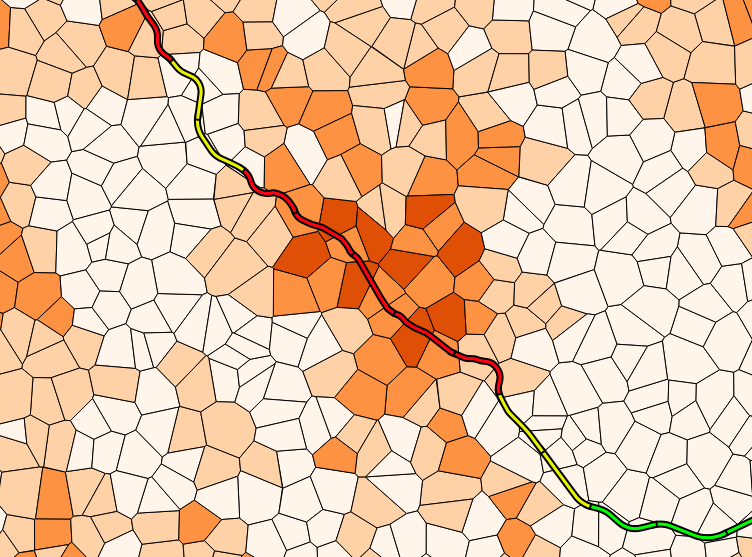
\includegraphics[width=0.6\textwidth]{images/rietizoom}
	\caption{$Km$ 13.5 della tratta Rieti - L'Aquila - Sulmona.}
	\label{km_13}
\end{figure}

\begin{figure}[h]
	\centering
	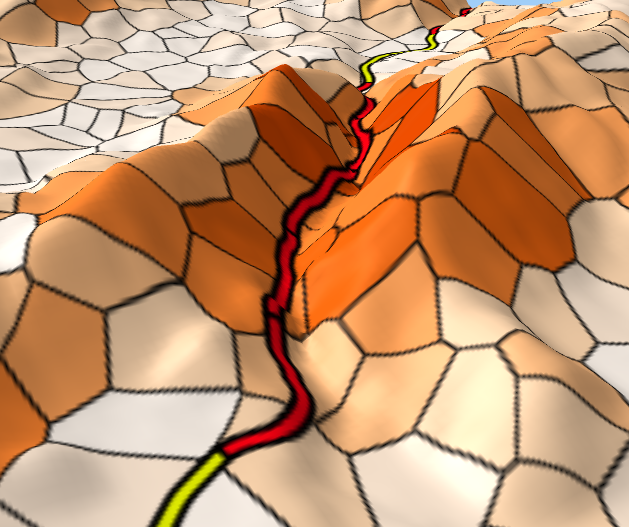
\includegraphics[width=0.6\textwidth]{images/rieti3d}
	\caption{Rendering 3D del $Km$ 13.5 della tratta Rieti - L'Aquila - Sulmona.}
	\label{km_13d}
\end{figure}


E' stata quindi calcolata la matrice di contingenza multi-classe (Tabella \ref{tab:MatriceContingenzaRoute}) e risulta che i valori più alti sono concentrati lungo la diagonale principale. Per questo motivo l'algoritmo ha eseguito una valutazione molto buona.

\begin{table}[H]
	\centering
	\renewcommand{\arraystretch}{1}
	\begin{tabular}{|c|C{2cm}|C{2cm}|C{2cm}|C{2cm}|c|}
		\hline
		\multicolumn{2}{|c|}{}                                                                                               & \multicolumn{3}{c|}{\textbf{Classi Stimate}}                                &                          \\ \cline{3-5}
		\multicolumn{2}{|c|}{\multirow{-2}{*}{}}                                                                                             & \cellcolor[HTML]{32CB00}Bassa & \cellcolor[HTML]{FFFE65}Media & \cellcolor[HTML]{FE0000}Alta & \multirow{-2}{*}{Totale} \\ \hline
		& \cellcolor[HTML]{32CB00}Bassa & 18                            & 2                             & 0                            & 20                       \\ \cline{2-6} 
		& \cellcolor[HTML]{FFFE65}Media & 2                             & 19                            & 0                            & 21                       \\ \cline{2-6} 
		\multirow{-3}{*}{\textbf{\begin{tabular}[c]{@{}c@{}}Classi\\ Reali\end{tabular}}} & \cellcolor[HTML]{FE0000}Alta  & 0                             & 0                            & 13                            & 13                        \\ \hline
		\multicolumn{2}{|c|}{Totale}                                                                                                         & 20                            & 21                            & 13                            & 54                      \\ \hline
	\end{tabular}
	\caption{\textit{matrice di contingenza multi-classe} delle sotto-tratte di Rieti - L'Aquila - Sulmona}
	\label{tab:MatriceContingenzaRoute}
\end{table} 

In particolare, per quanto riguarda la classe bassa, l’algoritmo riesce a valutare correttamente 18 sotto-tratte su 20. (Tabella \ref{tab:BinariaBassaRoute}).

\begin{table}[H]
	\centering
	\renewcommand{\arraystretch}{1}
	\begin{tabular}{|c|C{2cm}|C{2cm}|c|c|}
		\hline
		\multicolumn{2}{|c|}{}                                                                                                                  & \multicolumn{2}{c|}{\textbf{Classi Stimate}}    &                          \\ \cline{3-4}
		\multicolumn{2}{|c|}{\multirow{-2}{*}{}}                                                                                                & \cellcolor[HTML]{32CB00}Bassa & \cellcolor[HTML]{ECF4FF}No bassa & \multirow{-2}{*}{Totale} \\ \hline
		& \cellcolor[HTML]{32CB00}Bassa    & 18                            & 2                                & 20                       \\ \cline{2-5} 
		\multirow{-2}{*}{\textbf{\begin{tabular}[c]{@{}c@{}}Classi \\Reali\end{tabular}}} & \cellcolor[HTML]{ECF4FF}No bassa & 2                            & 32                               & 34                       \\ \hline
		\multicolumn{2}{|c|}{Totale}                                                 & 20                            & 34                               & 54                      \\ \hline
	\end{tabular}
	\caption{\textit{matrice di contingenza binaria} della classe a bassa pericolosità ricavata a partire dalla tabella di contingenza non binaria.}
	\label{tab:BinariaBassaRoute}
\end{table}

Per la classe media i risultati continuano ad essere molto buoni. L'algoritmo valuta correttamente 19 sotto-tratte su 21 (Tabella \ref{tab:BinariaMediaRoute}).

\begin{table}[H]
	\centering
	\renewcommand{\arraystretch}{1.2}
	\begin{tabular}{|c|C{2cm}|C{2cm}|c|c|}
		\hline
		\multicolumn{2}{|c|}{}                                                                                                                  & \multicolumn{2}{c|}{\textbf{Classi Stimate}}    &                          \\ \cline{3-4}
		\multicolumn{2}{|c|}{\multirow{-2}{*}{}}                                                                                                & \cellcolor[HTML]{FFFE65}Media & \cellcolor[HTML]{ECF4FF}No Media & \multirow{-2}{*}{Totale} \\ \hline
		& \cellcolor[HTML]{FFFE65}Media    & 19                            & 2                                & 21                       \\ \cline{2-5} 
		\multirow{-2}{*}{\textbf{\begin{tabular}[c]{@{}c@{}}Classi \\ Reali\end{tabular}}} & \cellcolor[HTML]{ECF4FF}No media & 2                             & 31                               & 33                       \\ \hline
		\multicolumn{2}{|c|}{Totale}                                                                                                            & 21                            & 33                               & 54                      \\ \hline
	\end{tabular}
	\caption{\textit{matrice di contingenza binaria} della classe a media pericolosità ricavata a partire dalla tabella di contingenza non binaria.}
	\label{tab:BinariaMediaRoute}
\end{table}

I risultati migliori si ottengono però per la classe alta. L'algoritmo valuta correttamente tutte e 13 le sotto-tratte (Tabella \ref{tab:BinariaAltaRoute}).

\begin{table}[H]
	\centering
	\renewcommand{\arraystretch}{1}
	\begin{tabular}{|c|C{2cm}|C{2cm}|c|c|}
		\hline
		\multicolumn{2}{|c|}{}                                                                                                                  & \multicolumn{2}{c|}{\textbf{Classi Stimate}}    &                          \\ \cline{3-4}
		\multicolumn{2}{|c|}{\multirow{-2}{*}{}}                                                                                                & \cellcolor[HTML]{FE0000}Alta & \cellcolor[HTML]{ECF4FF}No alta & \multirow{-2}{*}{Totale} \\ \hline
		& \cellcolor[HTML]{FE0000}Alta    & 13                           & 0                                & 13                       \\ \cline{2-5} 
		\multirow{-2}{*}{\textbf{\begin{tabular}[c]{@{}c@{}}Classi \\Reali\end{tabular}}} & \cellcolor[HTML]{ECF4FF}No alta & 0                             & 41                               & 41                       \\ \hline
		\multicolumn{2}{|c|}{Totale}                                                                                                            & 13                            & 41                               & 54                      \\ \hline
	\end{tabular}
	\caption{\textit{matrice di contingenza binaria} della classe ad alta pericolosità ricavata a partire dalla tabella di contingenza non binaria.}
	\label{tab:BinariaAltaRoute}
\end{table}
In tabella \ref{tab:RisultatiMetricheRoute} sono riassunti i risultati con le metriche già illustrate nel capitolo sei. 
In particolare per la classe alta si ottiene una precisione (P) e una accuratezza (ACC) entrambi massimi (pari a uno).
\begin{table}[h]
	\centering
	\renewcommand{\arraystretch}{1.2}
	\begin{tabular}{|C{3cm}|C{3cm}|C{3cm}|C{3cm}|}
		\hline
		\multicolumn{1}{|l|}{\cellcolor[HTML]{FFFFFF}} & \cellcolor[HTML]{32CB00}Bassa & \cellcolor[HTML]{FFFE65}Media & \cellcolor[HTML]{FE0000}Alta \\ \hline
		\textbf{TPR}                                   & 0,9                                                           & 0,9                                                           & 1                                                          \\ \hline
		\textbf{TNR}                                   & 0,94                                                           & 0,93                                                           & 1                                                          \\ \hline
		\textbf{P}                                     & 0,9                                                           & 0,9                                                           & 1                                                          \\ \hline
		\textbf{Acc}                                   & 0,92                                                           & 0,92                                                           & 1                                                          \\ \hline
	\end{tabular}
	\caption{ Fasce di pericolo con metriche (True Positive Rate, True Negative Rate, Precision, Accuracy) associate.}
	\label{tab:RisultatiMetricheRoute}
	\end{table}

\section{Archi Stazione - Atessa}
Nessuna delle tratte di Archi Stazione - Atessa appartene alla classe alta (Tabella \ref{exposure_archi_atessa}).

\begin{table}[H]
	\centering
	\begin{tabular}{|l|l|}
		\hline
		\rowcolor[HTML]{9B9B9B} 
		\multicolumn{1}{|c|}{\cellcolor[HTML]{9B9B9B}\textbf{Km}} & \multicolumn{1}{c|}{\cellcolor[HTML]{9B9B9B}\textbf{Exposure}} \\ \hline
		\rowcolor[HTML]{F8FF00} 
		13.5                                                      & 0.496843113                                                    \\ \hline
		\rowcolor[HTML]{F8FF00} 
		12                                                        & 0.440692262                                                    \\ \hline
		\rowcolor[HTML]{F8FF00} 
		9                                                         & 0.363006806                                                    \\ \hline
		\rowcolor[HTML]{F8FF00} 
		10.5                                                      & 0.354543437                                                    \\ \hline
		\rowcolor[HTML]{F8FF00} 
		7.5                                                       & 0.274951265                                                    \\ \hline
		\rowcolor[HTML]{F8FF00} 
		0                                                         & 0.273656919                                                    \\ \hline
		\rowcolor[HTML]{F8FF00} 
		1.5                                                       & 0.269139503                                                    \\ \hline
		\rowcolor[HTML]{32CB00} 
		6                                                         & 0.172300475                                                    \\ \hline
		\rowcolor[HTML]{32CB00} 
		3                                                         & 0.136815565                                                    \\ \hline
		\rowcolor[HTML]{32CB00} 
		4.5                                                       & 0.128632086                                                    \\ \hline
	\end{tabular}
	\caption{Exposure sotto-tratte Archi Stazione - Atessa.}
	\label{exposure_archi_atessa}
\end{table}
Nessun punto delle sotto-tratte appartiene alla classe alta (Tabella \ref{risultati_archi_atessa}).

\begin{table}[H]
	\centering
	\begin{tabular}{|c|c|c|}
		\hline
		\rowcolor[HTML]{C0C0C0} 
		\textbf{Exposure} & \textbf{\# hotspot} & \textbf{\% di hotspot per exposure} \\ \hline
		Classe Alta       & 0                  & 0                                  \\ \hline
		Classe Media      & 26                 & 65                        \\ \hline
		Classe Bassa      & 14              & 35                            \\ \hline
		Tot. Hotspot      & 40               & 100                                 \\ \hline
	\end{tabular}
	\caption{Classi di expsure dei punti delle sotto-tratte Archi Stazione - Atessa.}
	\label{risultati_archi_atessa}
\end{table}

Risulta quindi che per l'algoritmo la tratta non è pericolosa. 